\chapter{Realization: Main setup}
\minitoc
\newpage

\setcounter{secnumdepth}{0} % Set the section counter to 0 so next section is not counted in toc
% ----------------------- Introduction ----------------------- %
\section{Introduction}
In this chapter, we will finally discuss the long awaited realization.
This is the implementation phase where all of the work done in the previous chapters comes into picture.
This section will {\bf heavily focus on DevOps} since our primary objective has been migrating the \glsxtrshort{ilg} application to a new scalable architecture using modern DevOps standards.
We will start with the new architecture hardware and software setup then talk about how to monitor the whole application stack.

\setcounter{secnumdepth}{2} % Resume counting the sections for the toc with a depth of 2 (Sections and sub-sections)
% ----------------------- Hardware setup ----------------------- %
\section{Hardware setup}
Since we agreed to proceed with the self-managed Kubernetes deployment as mentioned in \textbf{Chapter 2: State of the art}, we must create our own cluster nodes or virtual machines.
The nodes in question can be separated into the core nodes that are create once, and the scalable nodes that can be created indefinitely whenever we need to scale.

\subsection{Cloud provider}
To provision the hardware resources that we need for the deployment, we're going  to use the IONOS Cloud provider.
\cite[Ionos is a web hosting company founded in Germany in 1988 and is currently owned by United Internet.]{ionos-wikipedia}
\begin{figure}[H]
    \centering
    \makebox[\textwidth]{
\includegraphics[width=8cm]{src/assets/images/ionos-logo.png}}
    \caption{Logo of IONOS}
    \label{fig:logo-of-ionos-cloud}
\end{figure}

IONOS Cloud provides -through the Ionos cloudpanel service- an easy way to create and manage virtual machines, firewall rules, private networks and various other infrastructure components.
\begin{figure}[H]
    \centering
    \makebox[\textwidth]{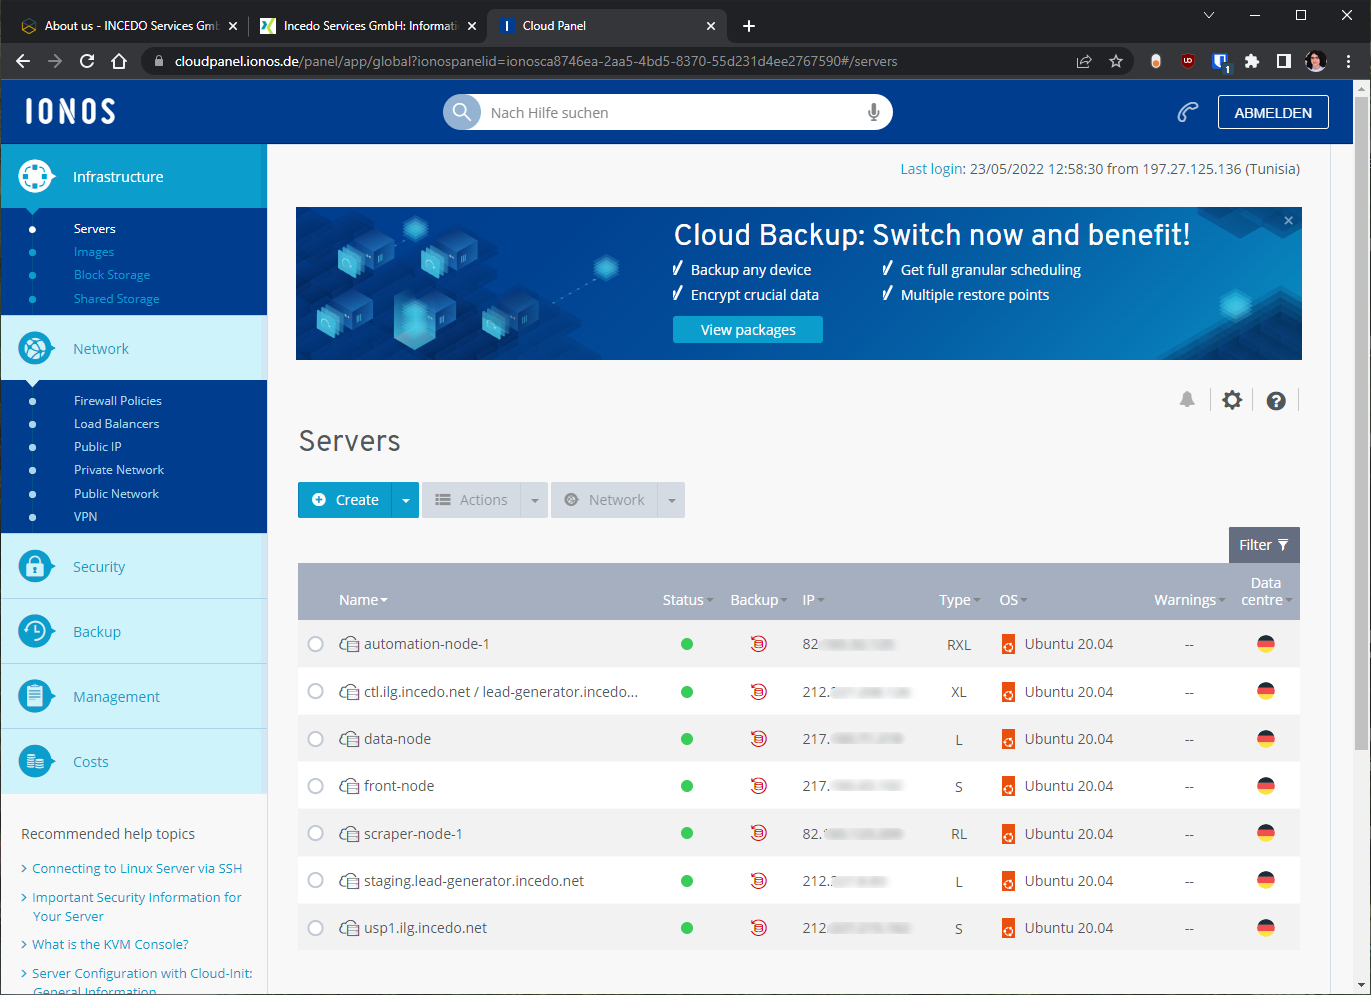
\includegraphics[width=\linewidth]{src/assets/images/ionos-cloudpanel-dashboard.JPG}}
    \caption{Ionos cloudpanel dashboard}
    \label{fig:image-of-ionos-cloudpanel-dashboard}
\end{figure}

The dashboard options of IONOS cloudpanel we use during our deployment process are:

\textbf{Infrastructure:}
\begin{itemize}
    \item \textbf{Server:} To create and manage our virtual machines.
    \item \textbf{Block storage:} To create and connect an SSD to a single server for extra storage.
\end{itemize}

\textbf{Network:}
\begin{itemize}
    \item \textbf{Firewall Policies:} To create firewall rules to protect our VMs.
    \item \textbf{Private Network:} To create and manage private networks for server to server communication.
\end{itemize}

The two images below show the available \glsxtrshort{vm} sizes in the Ionos cloudpanel dashboard and their corresponding specifications.
We will refer to the sizes in the tables of the next section.
\begin{figure}[H]
    \centering
    \makebox[\textwidth]{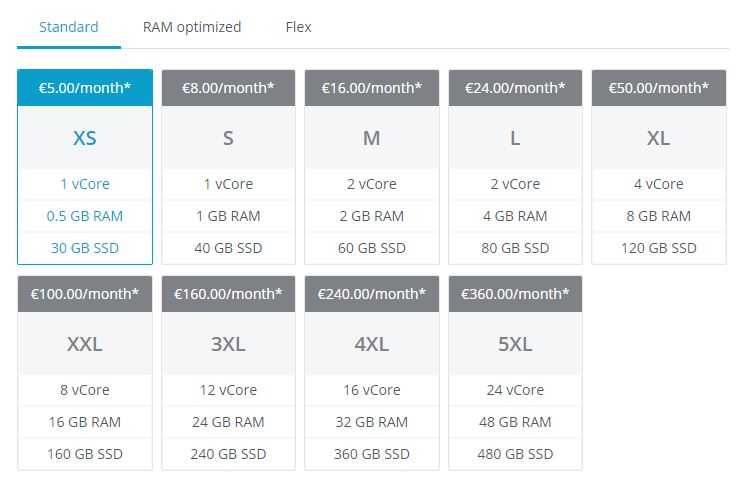
\includegraphics[width=\linewidth]{src/assets/images/vm-standard.jpg}}
    \caption{Standard VM sizes in IONOS}
    \label{fig:standard-vm-sizes}
\end{figure}
\begin{figure}[H]
    \centering
    \makebox[\textwidth]{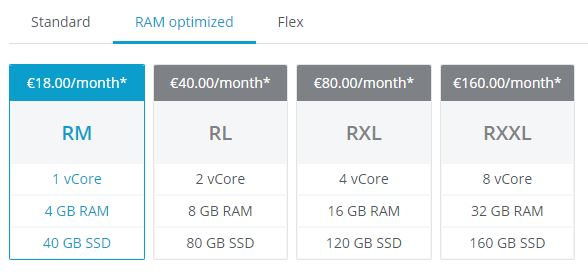
\includegraphics[width=\linewidth]{src/assets/images/vm-ram-optimized.JPG}}
    \caption{RAM Optimized VM sizes in IONOS}
    \label{fig:ram-optimized-vm-sizes}
\end{figure}

\subsection{Kubernetes Cluster}
Using the cloudpanel dashboard, it is time that we setup our cluster.
The tables below show the virtual machines that we need to get started.

\begin{table}[H]
    \renewcommand{\arraystretch}{1.5} % Padding
    \caption{Core cluster nodes}
    \centering
    \medskip
    \begin{tabularx}{1\textwidth} {
            | >{\hsize=1\hsize\linewidth=\hsize\raggedright\arraybackslash}X
            | >{\hsize=1.8\hsize\linewidth=\hsize\raggedright\arraybackslash}X
            | >{\hsize=0.2\hsize\linewidth=\hsize\centering\arraybackslash}X |}
        \hline
        \rowcolor{primary} \textbf{Name} & \textbf{Services}                            & \textbf{Size} \\
        \hline
        \textbf{kube-controller}         & The main Kubernetes cluster controller       & XL            \\
        \hline
        \textbf{data-node}               & PostgresDB, ilg-data, ilg-api, ilg-scheduler & L             \\
        \hline
        \textbf{front-node}              & ilg-front                                    & S             \\
        \hline
        \textbf{staging-node}            & PostgresDB, all other ilg services           & L             \\
        \hline
    \end{tabularx}
\end{table}

\begin{table}[H]
    \renewcommand{\arraystretch}{1.5} % Padding
    \caption{Scalable cluster nodes}
    \centering
    \medskip
    \begin{tabularx}{1\textwidth} {
            | >{\hsize=1.2\hsize\linewidth=\hsize\raggedright\arraybackslash}X
            | >{\hsize=1.5\hsize\linewidth=\hsize\raggedright\arraybackslash}X
            | >{\hsize=0.3\hsize\linewidth=\hsize\centering\arraybackslash}X |}
        \hline
        \rowcolor{primary} \textbf{Name} & \textbf{Services} & \textbf{Size} \\
        \hline
        \textbf{scraper-node-n}          & ilg-scraper       & RL            \\
        \hline
        \textbf{automation-node-n}       & ilg-automation    & RXL           \\
        \hline
    \end{tabularx}
\end{table}

Please note that
\begin{itemize}
    \item What each of the services represent is already mentioned in \textbf{Chapter 3: Analysis and specification of requirements}
    \item The size column which stands for the specification of the virtual machine is described in the previous section.
    \item The number of servers for \textbf{scraper}, and \textbf{automation} nodes will be scaled manually depending on the number of clients whenever the need arises.
\end{itemize}

\subsection{Proxy Servers}
Proxies are used to ensure all requests to LinkedIn come from a single IP address in order to avoid having to write a verification code every time.
\begin{table}[H]
    \renewcommand{\arraystretch}{1.5} % Padding
    \caption{List of proxy servers}
    \centering
    \medskip
    \begin{tabularx}{1\textwidth} {
            | >{\hsize=1\hsize\linewidth=\hsize\raggedright\arraybackslash}X
            | >{\hsize=1.8\hsize\linewidth=\hsize\raggedright\arraybackslash}X
            | >{\hsize=0.2\hsize\linewidth=\hsize\centering\arraybackslash}X |}
        \hline
        \rowcolor{primary} \textbf{Name} & \textbf{Services}                   & \textbf{Size} \\
        \hline
        \textbf{usp-n}                   & Upstream proxy server running Squid & XS            \\
        \hline
    \end{tabularx}
\end{table}

\newpage
% ----------------------- Software setup ----------------------- %
\section{Software setup}
After setting up our hardware resources, we end up with raw Linux virtual machines with no configuration whatsoever.
We have to create and manage our own Kubernetes instance on it to proceed any further.
We will be using {\bf MicroK8s}.
But before that, we also need to setup some basic configuration.

\subsection{Manual configuration}
For a single virtual machine, we have to do the following setup:

\begin{itemize}
    \item Create a user with sudo permissions
    \item Install the base packages we will be using
    \item Edit the hosts file so that the virtual machine recognizes the other virtual machines by their hostnames
    \item Install MicroK8s to have a single-node cluster running on the virtual machine
    \item Join the virtual machine with the master node to have a multi-node cluster.
\end{itemize}

\subsection{Automating the process}
Manually configuring the above can be extremely tedious, inefficient and error prone.
Therefore, we've created {\bf Ansible} scripts or playbooks that do just that. In the end, we simply edit a configuration file and directly run the script.
This has a huge advantage especially when
\begin{itemize}
    \item We want to create a development environment for easy prototyping.
    \item We want to use the exact same setup for future projects.
    \item We want to add nodes to the cluster later on when scaling.
\end{itemize}

The playbook in question should first of all, apply the common configuration to all nodes.
Second of all, it should install MicroK8s on all nodes.
After that, it needs to configure the master node appropriately.
Finally, it configures the other nodes to join the cluster as worker nodes so that they can execute our services.

There are more details related to Kubernetes such as node tainting and node selectors that won't be mentioned  in this report due to time constraints.

Also note that we won't get into too much details about how Ansible works in this report also due to time constraints and since it will become very lengthy. We'll only mention that the connection is established using SSH.

\begin{figure}[H]
    \centering
    \makebox[\textwidth]{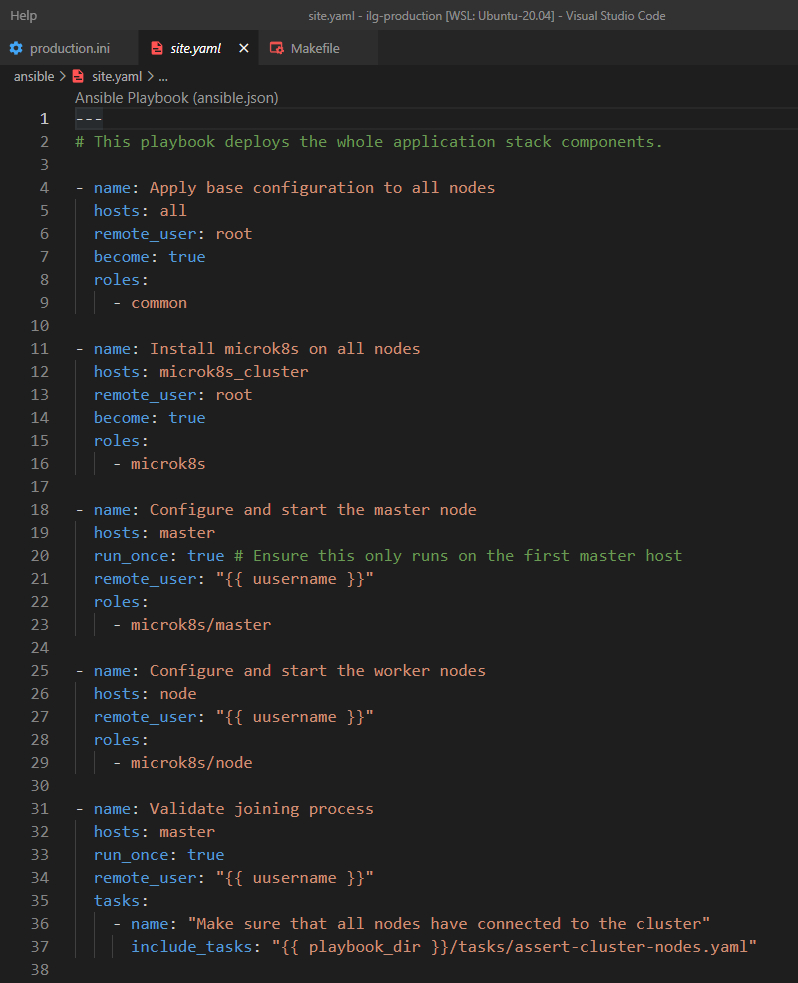
\includegraphics[width=13cm]{src/assets/images/ansible-main-script.JPG}}
    \caption{Extract from the Ansible playbook}
    \label{fig:extract-from-ansible-playbook}
\end{figure}

\begin{figure}[H]
    \centering
    \makebox[\textwidth]{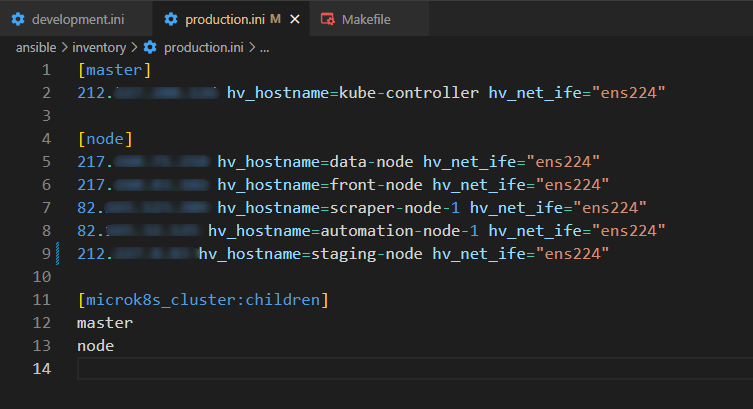
\includegraphics[width=\linewidth]{src/assets/images/ansible-hosts.JPG}}
    \caption{The Ansible hosts configuration}
    \label{fig:image-of-ansible-hosts}
\end{figure}
Note that we also use a hosts file for development where we test the setup extensively before trying it on production as seen from the figure just above.

% ----------------------- Application pipeline ----------------------- %
\section{Deployment process}
We will now explain the approach we adopted to continuously integrate, deploy and deliver our application as per the best practices of DevOps previously mentioned in \textbf{Chapter 3: State of the art}.
The deployment is currently supported on two different environments; the staging environment where we make sure our application works as intended, and of course the production environment.

\subsection{Adopted strategy}
Since we have multiple microservices, it would not be ideal to interact with our Kubernetes cluster from all of them whenever we make a change.
For that reason we use the following steps to deploy our application.
\begin{itemize}
    \item On code changes on any microservice, we create a new Docker image that we push to a custom container registry.
    \item Once the build is finished, we trigger a multi-project pipeline to a central repository we will call ilg-controller.
    \item The central repository will interact with our Kubernetes cluster to make the final deployment to the correct environment using a custom Helm package that we create.
\end{itemize}

This is further explained in detail in the following sub sections.

\subsection{Linking the cluster to GitLab}
Since we have a Kubernetes cluster and we also use GitLab, we will link the two using the GitLab Kubernetes Agent, or KAS for short.

\begin{figure}[H]
    \centering
    \makebox[\textwidth]{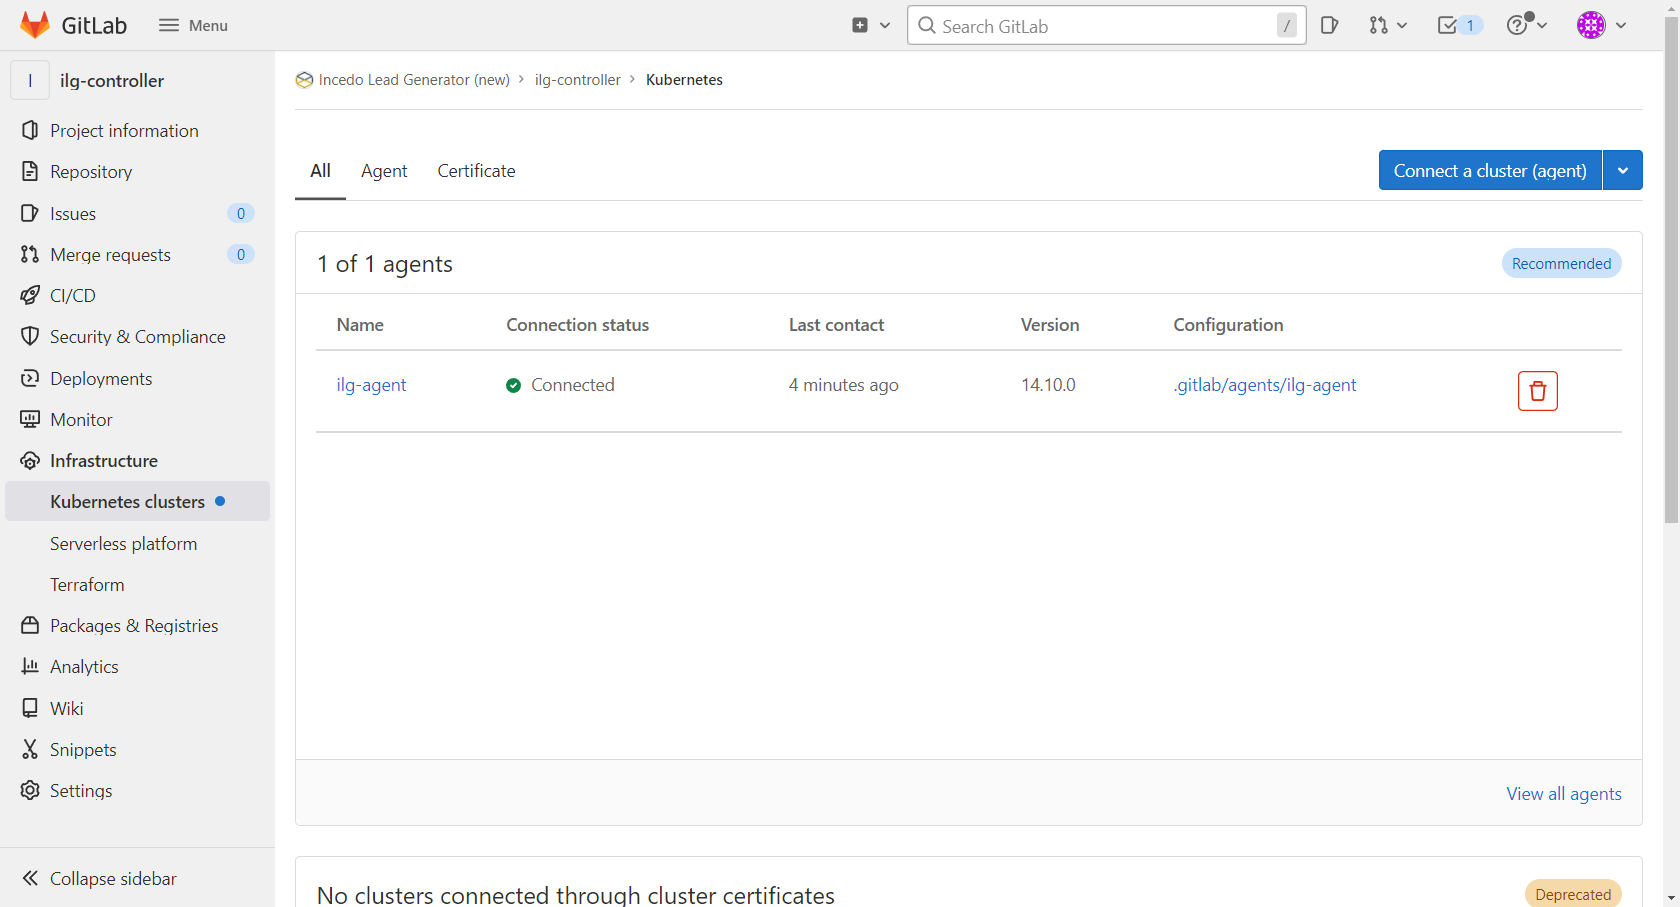
\includegraphics[width=\linewidth]{src/assets/images/gitlab-kubernetes-agent.JPG}}
    \caption{GitLab Kubernetes Agent}
    \label{fig:gitlab-kubernetes-agent}
\end{figure}

% CI Continuous Integration
\subsection{Continuous Integration}
When we as developers make code changes to the main branch of any microservice, tests are automatically executed.
If the tests are validated, a new Docker image that incorporates the changes we make will be pushed to the container registry and our deployment pipeline will then be triggered.
In other words, the new code will be integrated and that actually marks the end of this step.
\begin{figure}[H]
    \centering
    \makebox[\textwidth]{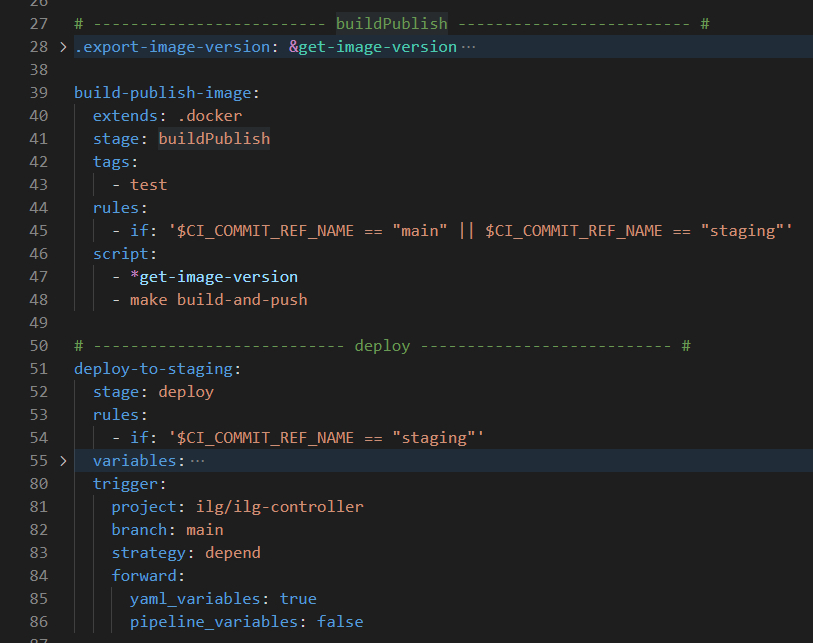
\includegraphics[width=10cm]{src/assets/images/ci-pipeline-extract.JPG}}
    \caption{Extract from the CI pipeline}
    \label{fig:extract-from-ci-pipeline}
\end{figure}

% CD Continuous Deployment
\subsection{Continuous Deployment}
Our ilg-controller repository (where the agent is configured) chooses the correct microservice to deploy depending on the trigger input.
It then sets the necessary environment variables for it and installs it using a custom Helm package we've created for the deployment.

\begin{figure}[H]
    \centering
    \makebox[\textwidth]{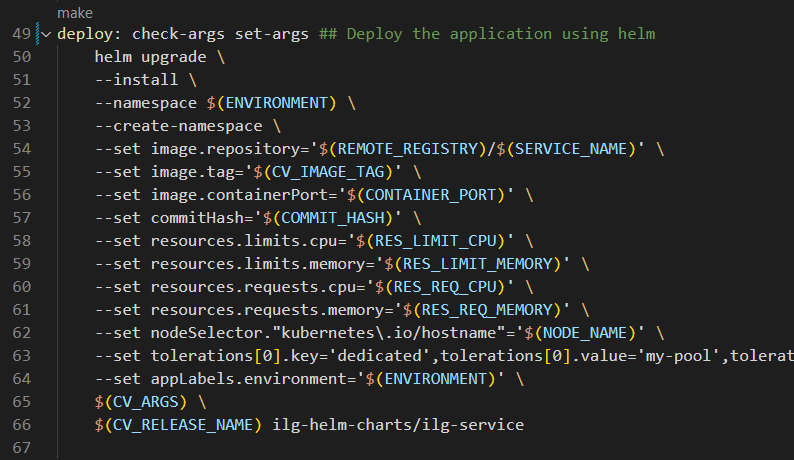
\includegraphics[width=11cm]{src/assets/images/cd-makefile-extract.JPG}}
    \caption{Extract from the deployment Makefile}
    \label{fig:extract-from-cd-makefile}
\end{figure}

% NOTE: Continuous delivery is a partly manual process where developers can deploy any changes to customers by simply clicking a button, while continuous deployment emphasizes automating the entirety of the process.

% Custom Helm Package
\subsection{Custom Helm Package}
Since we agreed to use Helm (refer to \textbf{Chapter 2: State of the art}), we've created a package -or in terms of Helm- a chart of our own to manage the Kubernetes cluster resources.

\begin{figure}[H]
    \centering
    \makebox[\textwidth]{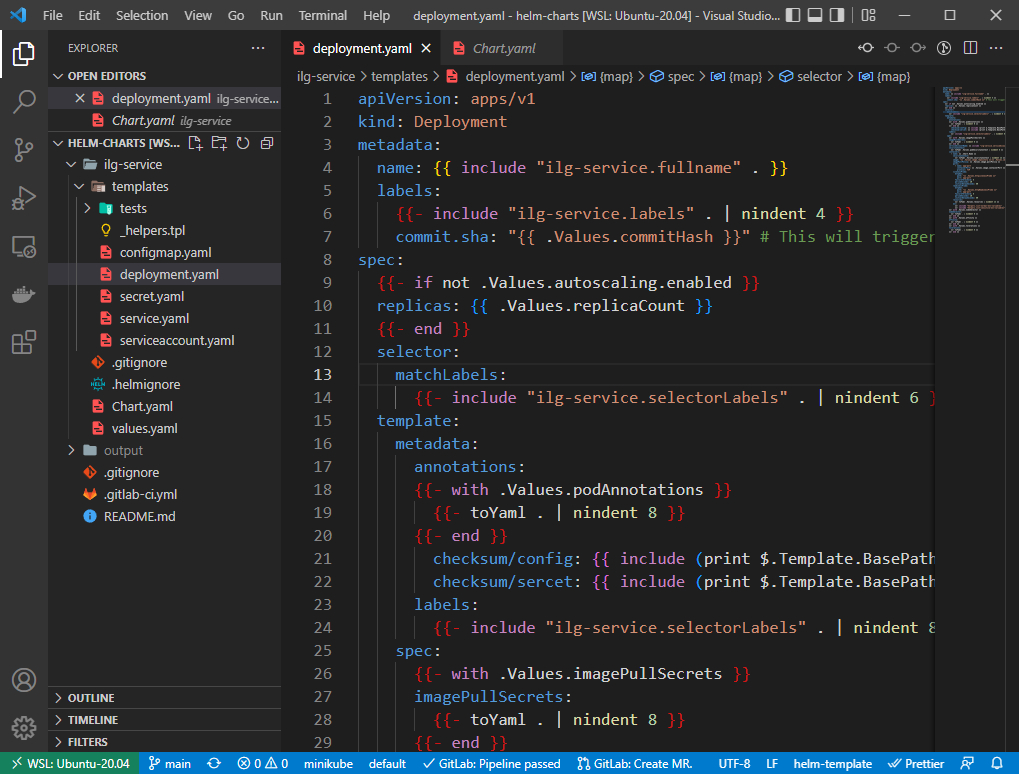
\includegraphics[width=15cm]{src/assets/images/helm-chart-code-extract.JPG}}
    \caption{Extract from the custom Helm Chart}
    \label{fig:extract-from-custom-helm-chart}
\end{figure}

We even integrate a CI/CD pipeline for the Helm chart itself so that new packages are built automatically whenever we make changes to the manifest template files.

\begin{figure}[H]
    \centering
    \makebox[\textwidth]{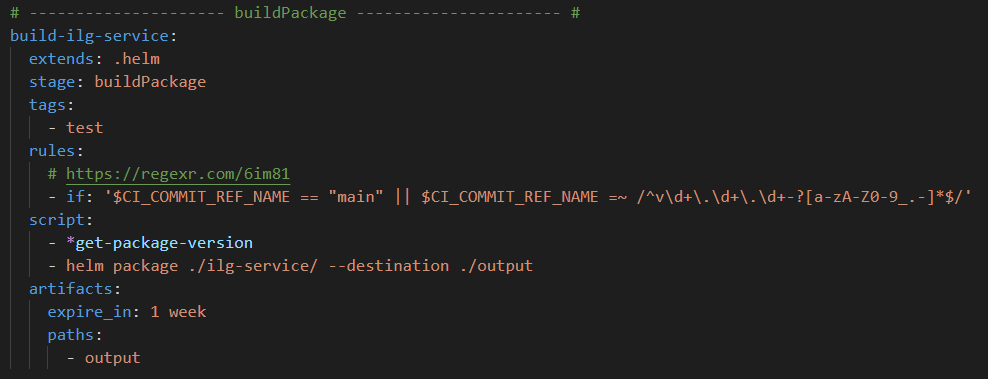
\includegraphics[width=15cm]{src/assets/images/build-pacakge-stage.JPG}}
    \caption{Extract from the custom Helm package's pipeline}
    \label{fig:build-package-stage}
\end{figure}

\begin{figure}[H]
    \centering
    \makebox[\textwidth]{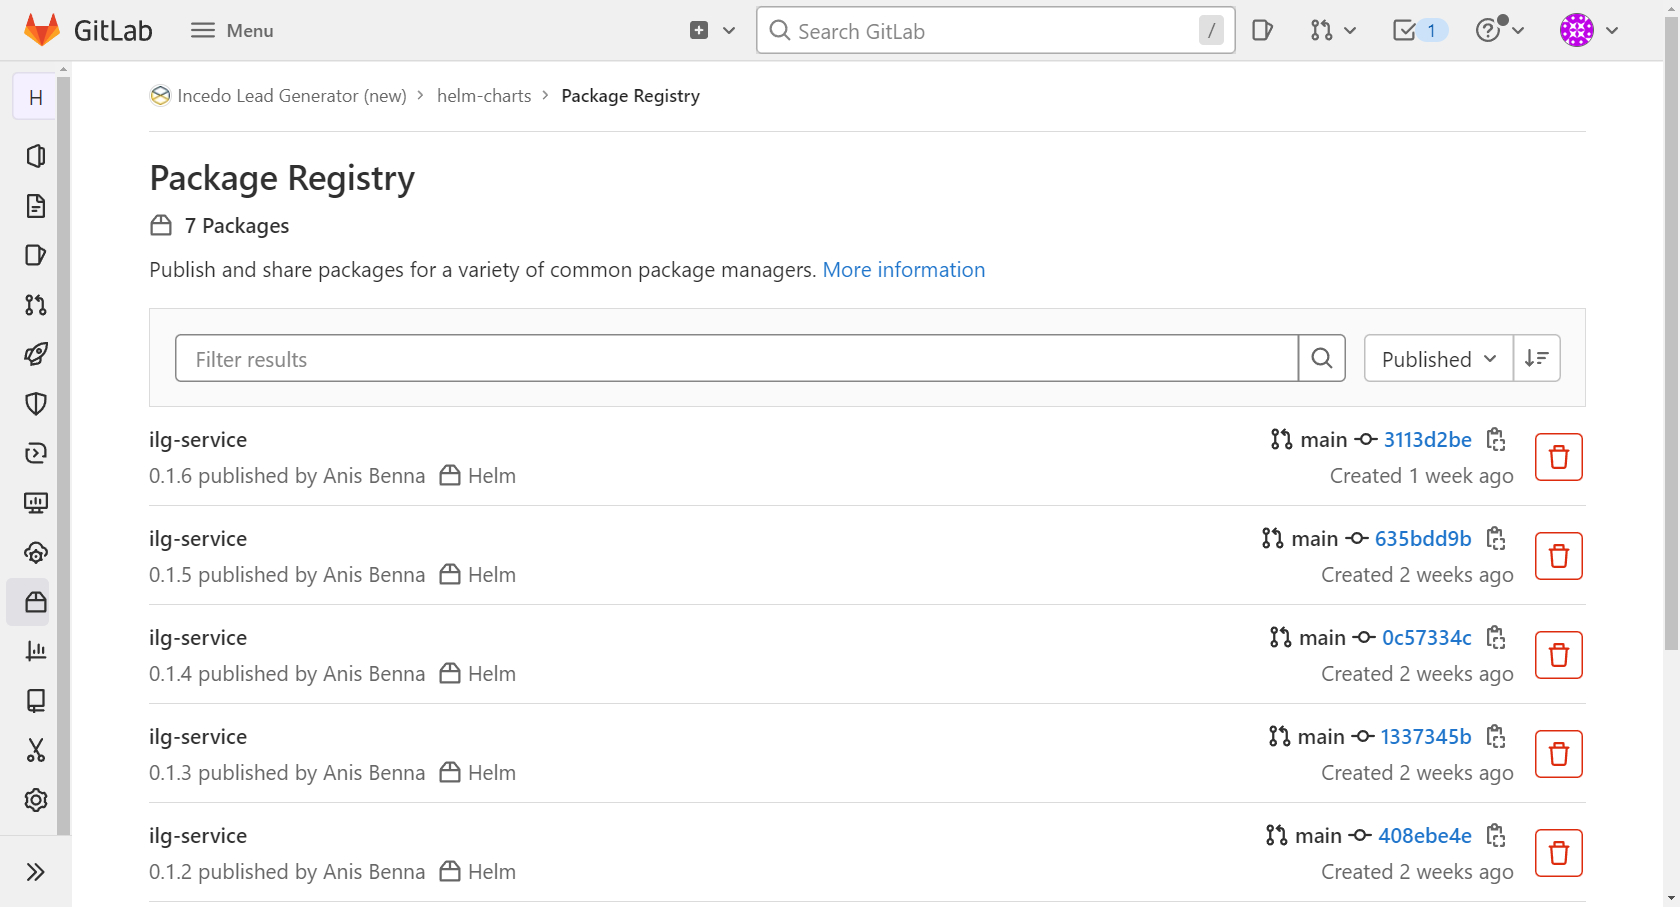
\includegraphics[width=15cm]{src/assets/images/gitlab-package-registry.JPG}}
    \caption{GitLab's package registry}
    \label{fig:gitlab-package-registry}
\end{figure}
\newpage

\subsection{Deployment result}
And now if we trigger the CI/CD pipeline of all of our microservices (please see \textbf{Appendix c}), we can see the application dashboard deployed!
In fact, we now have two live environments that are publicly available:
\begin{itemize}
    \item \textbf{Production:} \url{https://lead-generator.incedo.net}
    \item \textbf{Staging:} \url{https://staging.lead-generator.incedo.net}
\end{itemize}

\begin{figure}[H]
    \centering
    \makebox[\textwidth]{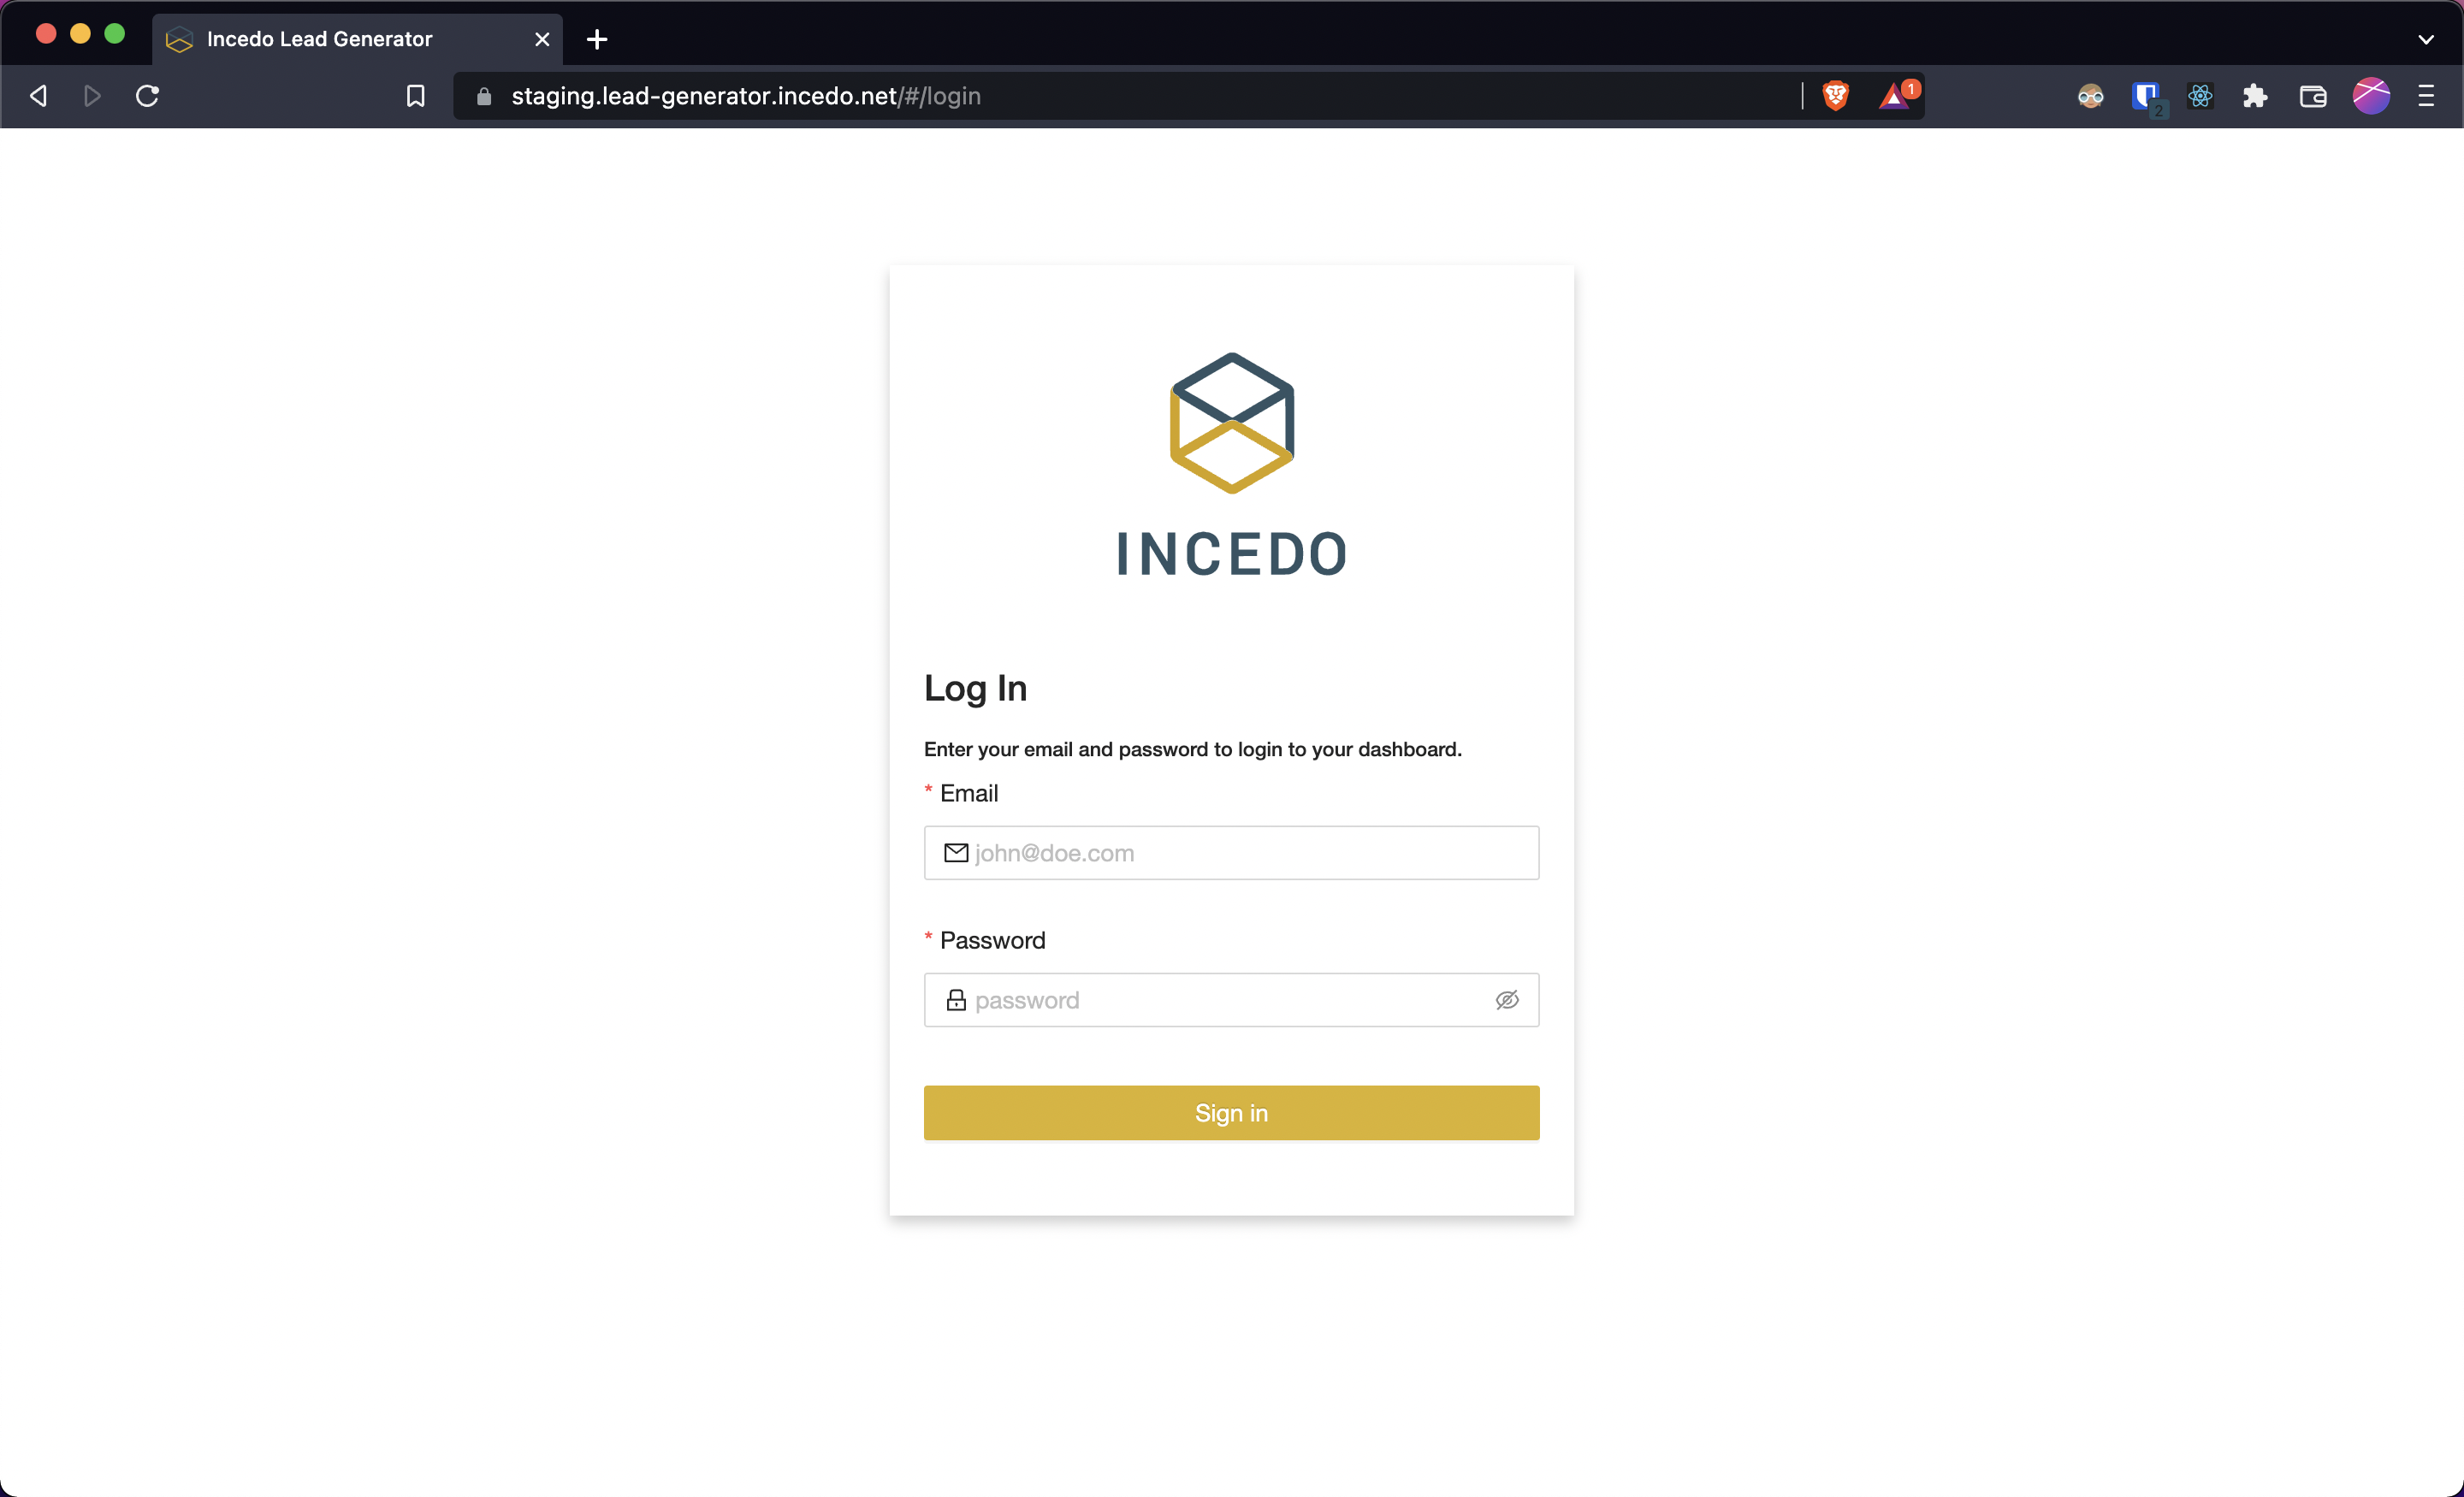
\includegraphics[width=\linewidth]{src/assets/app-screenshots/login.png}}
    \caption{ILG Login page}
    \label{fig:login-page}
\end{figure}

When we login, the dashboard with the list of campaigns is the first thing we notice. We can see how many active or inactive campaigns we have and also some useful statistics about how well our campaigns are doing.

We can also manage our campaigns by adding, editing or deleting them as per the defined requirements.
See \textbf{Appendix a} for more details.
\begin{figure}[H]
    \centering
    \makebox[\textwidth]{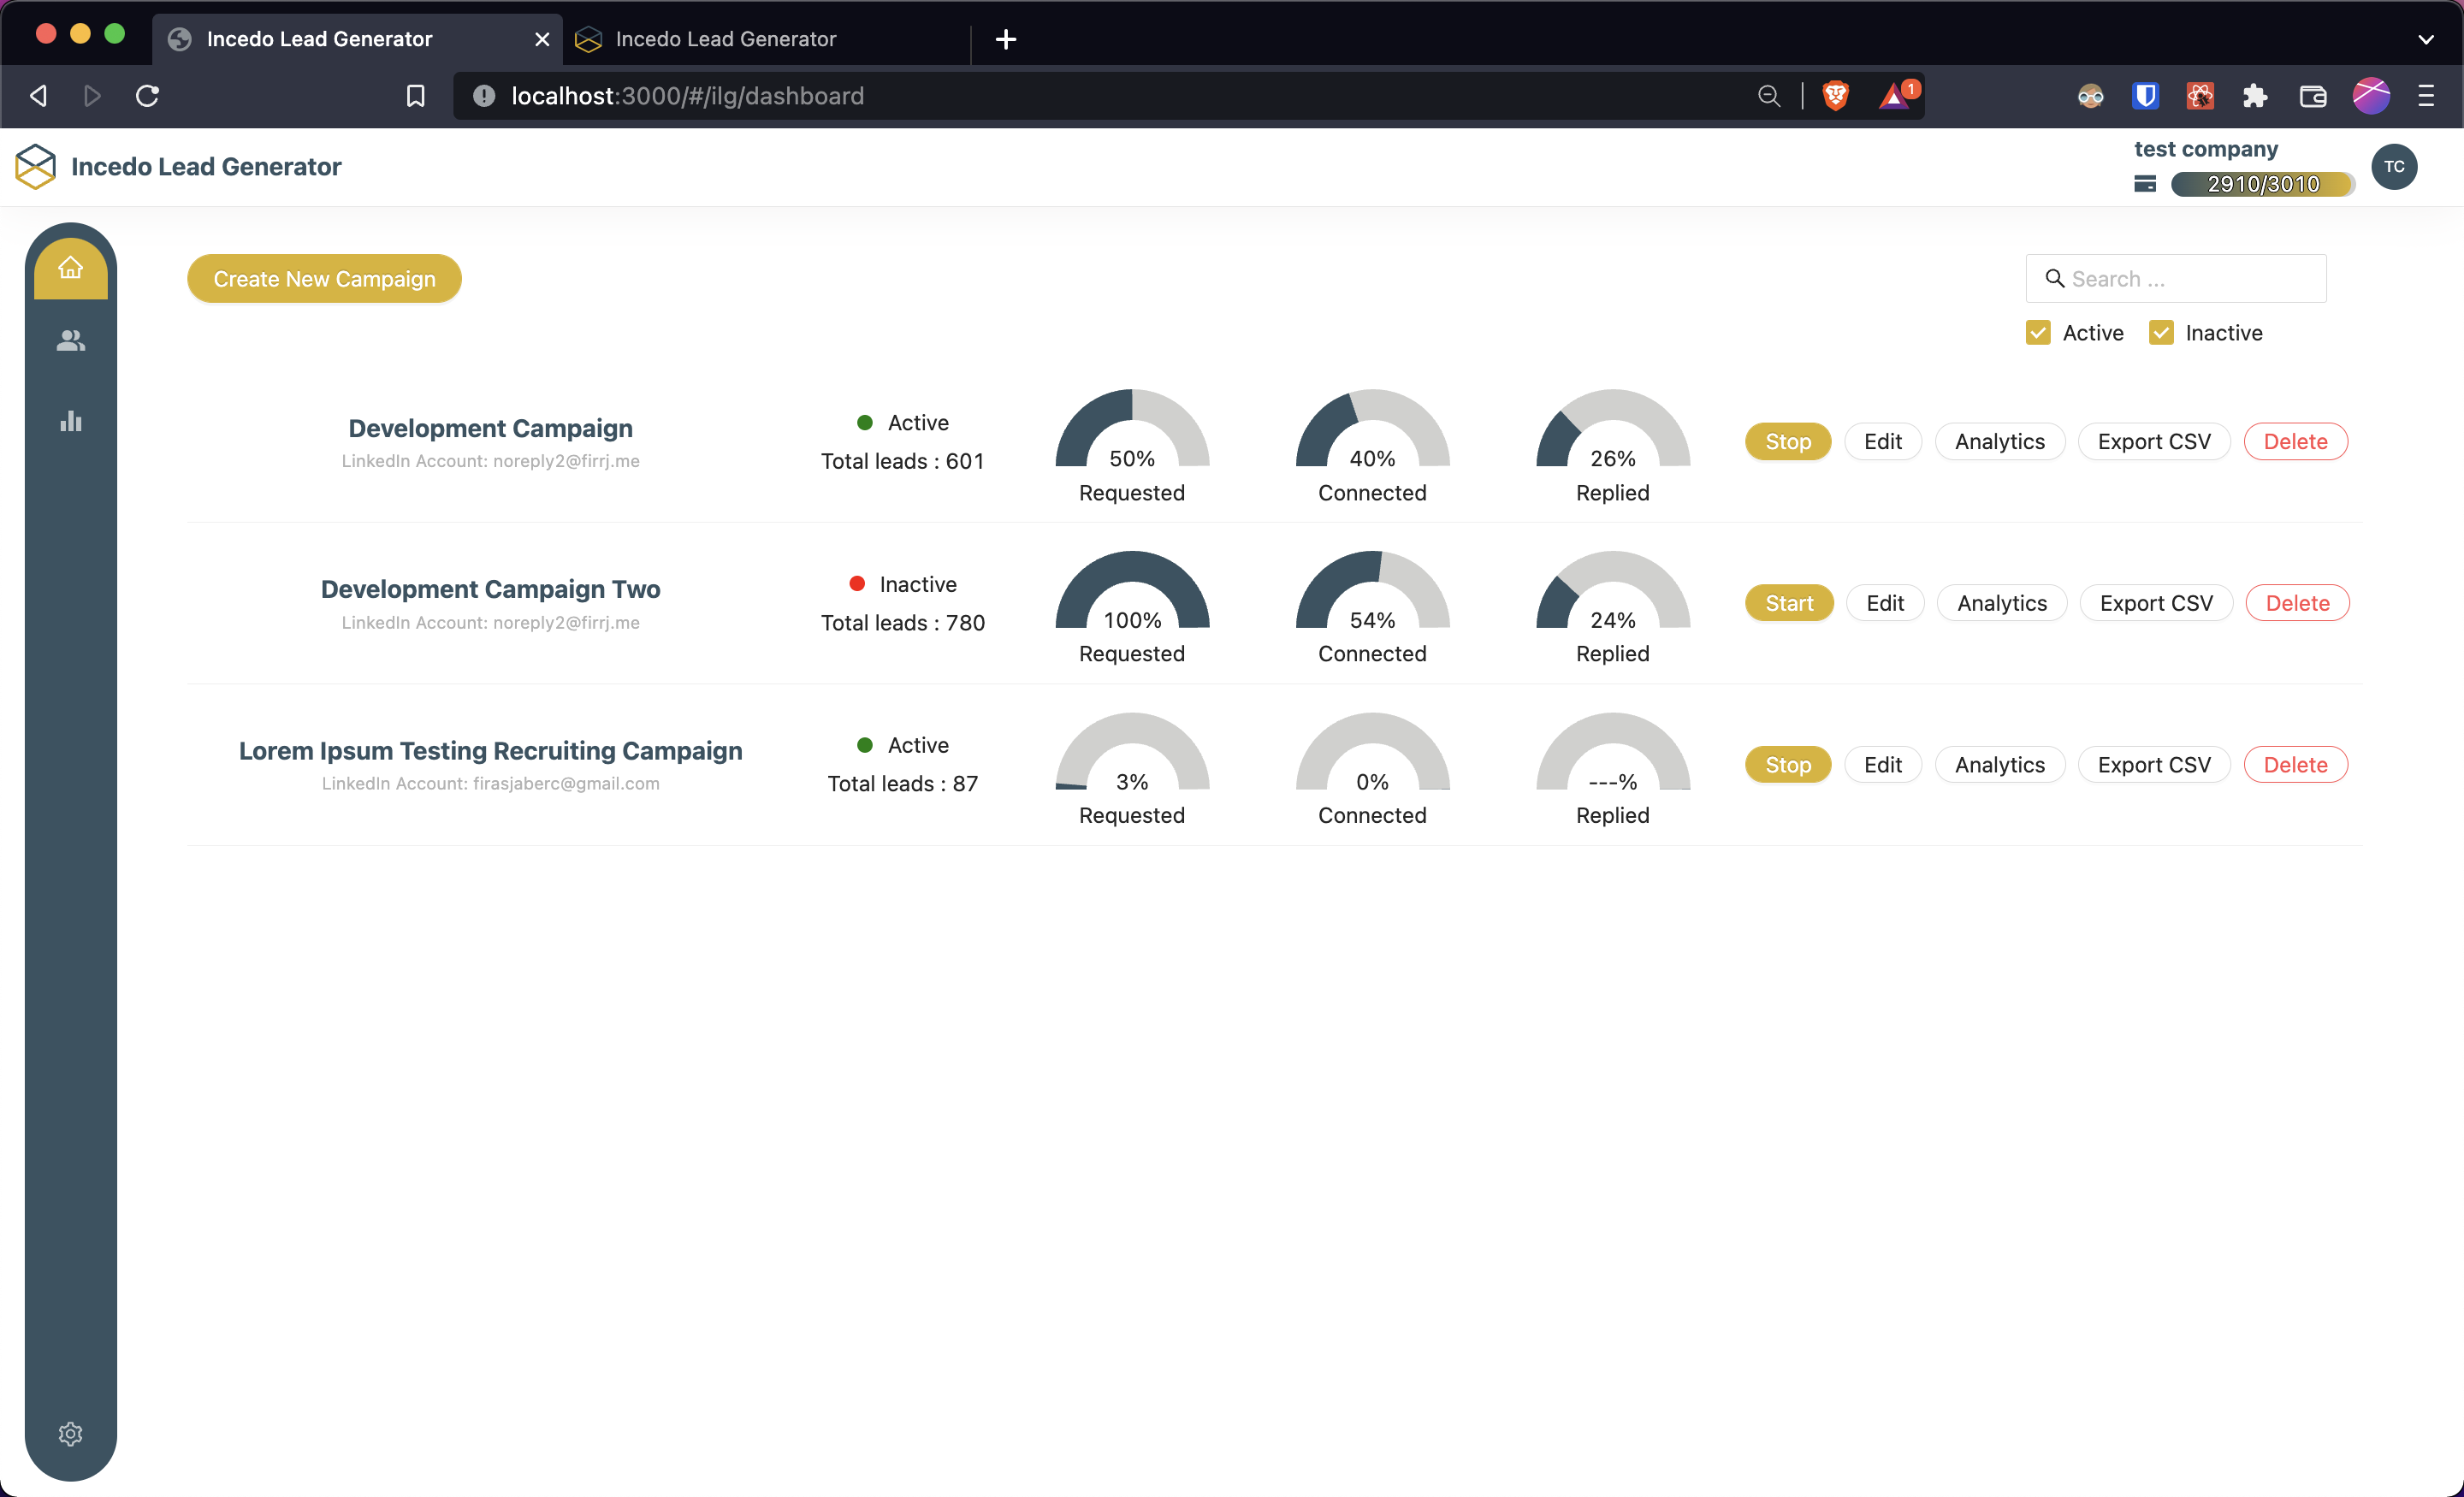
\includegraphics[width=\linewidth]{src/assets/app-screenshots/campaigns.png}}
    \caption{Campaigns overview page}
    \label{fig:campaigns-overview}
\end{figure}

We additionally have the option to manage our users as well as their credits.
Also refer to \textbf{Appendix b} for more screenshots.
\begin{figure}[H]
    \centering
    \makebox[\textwidth]{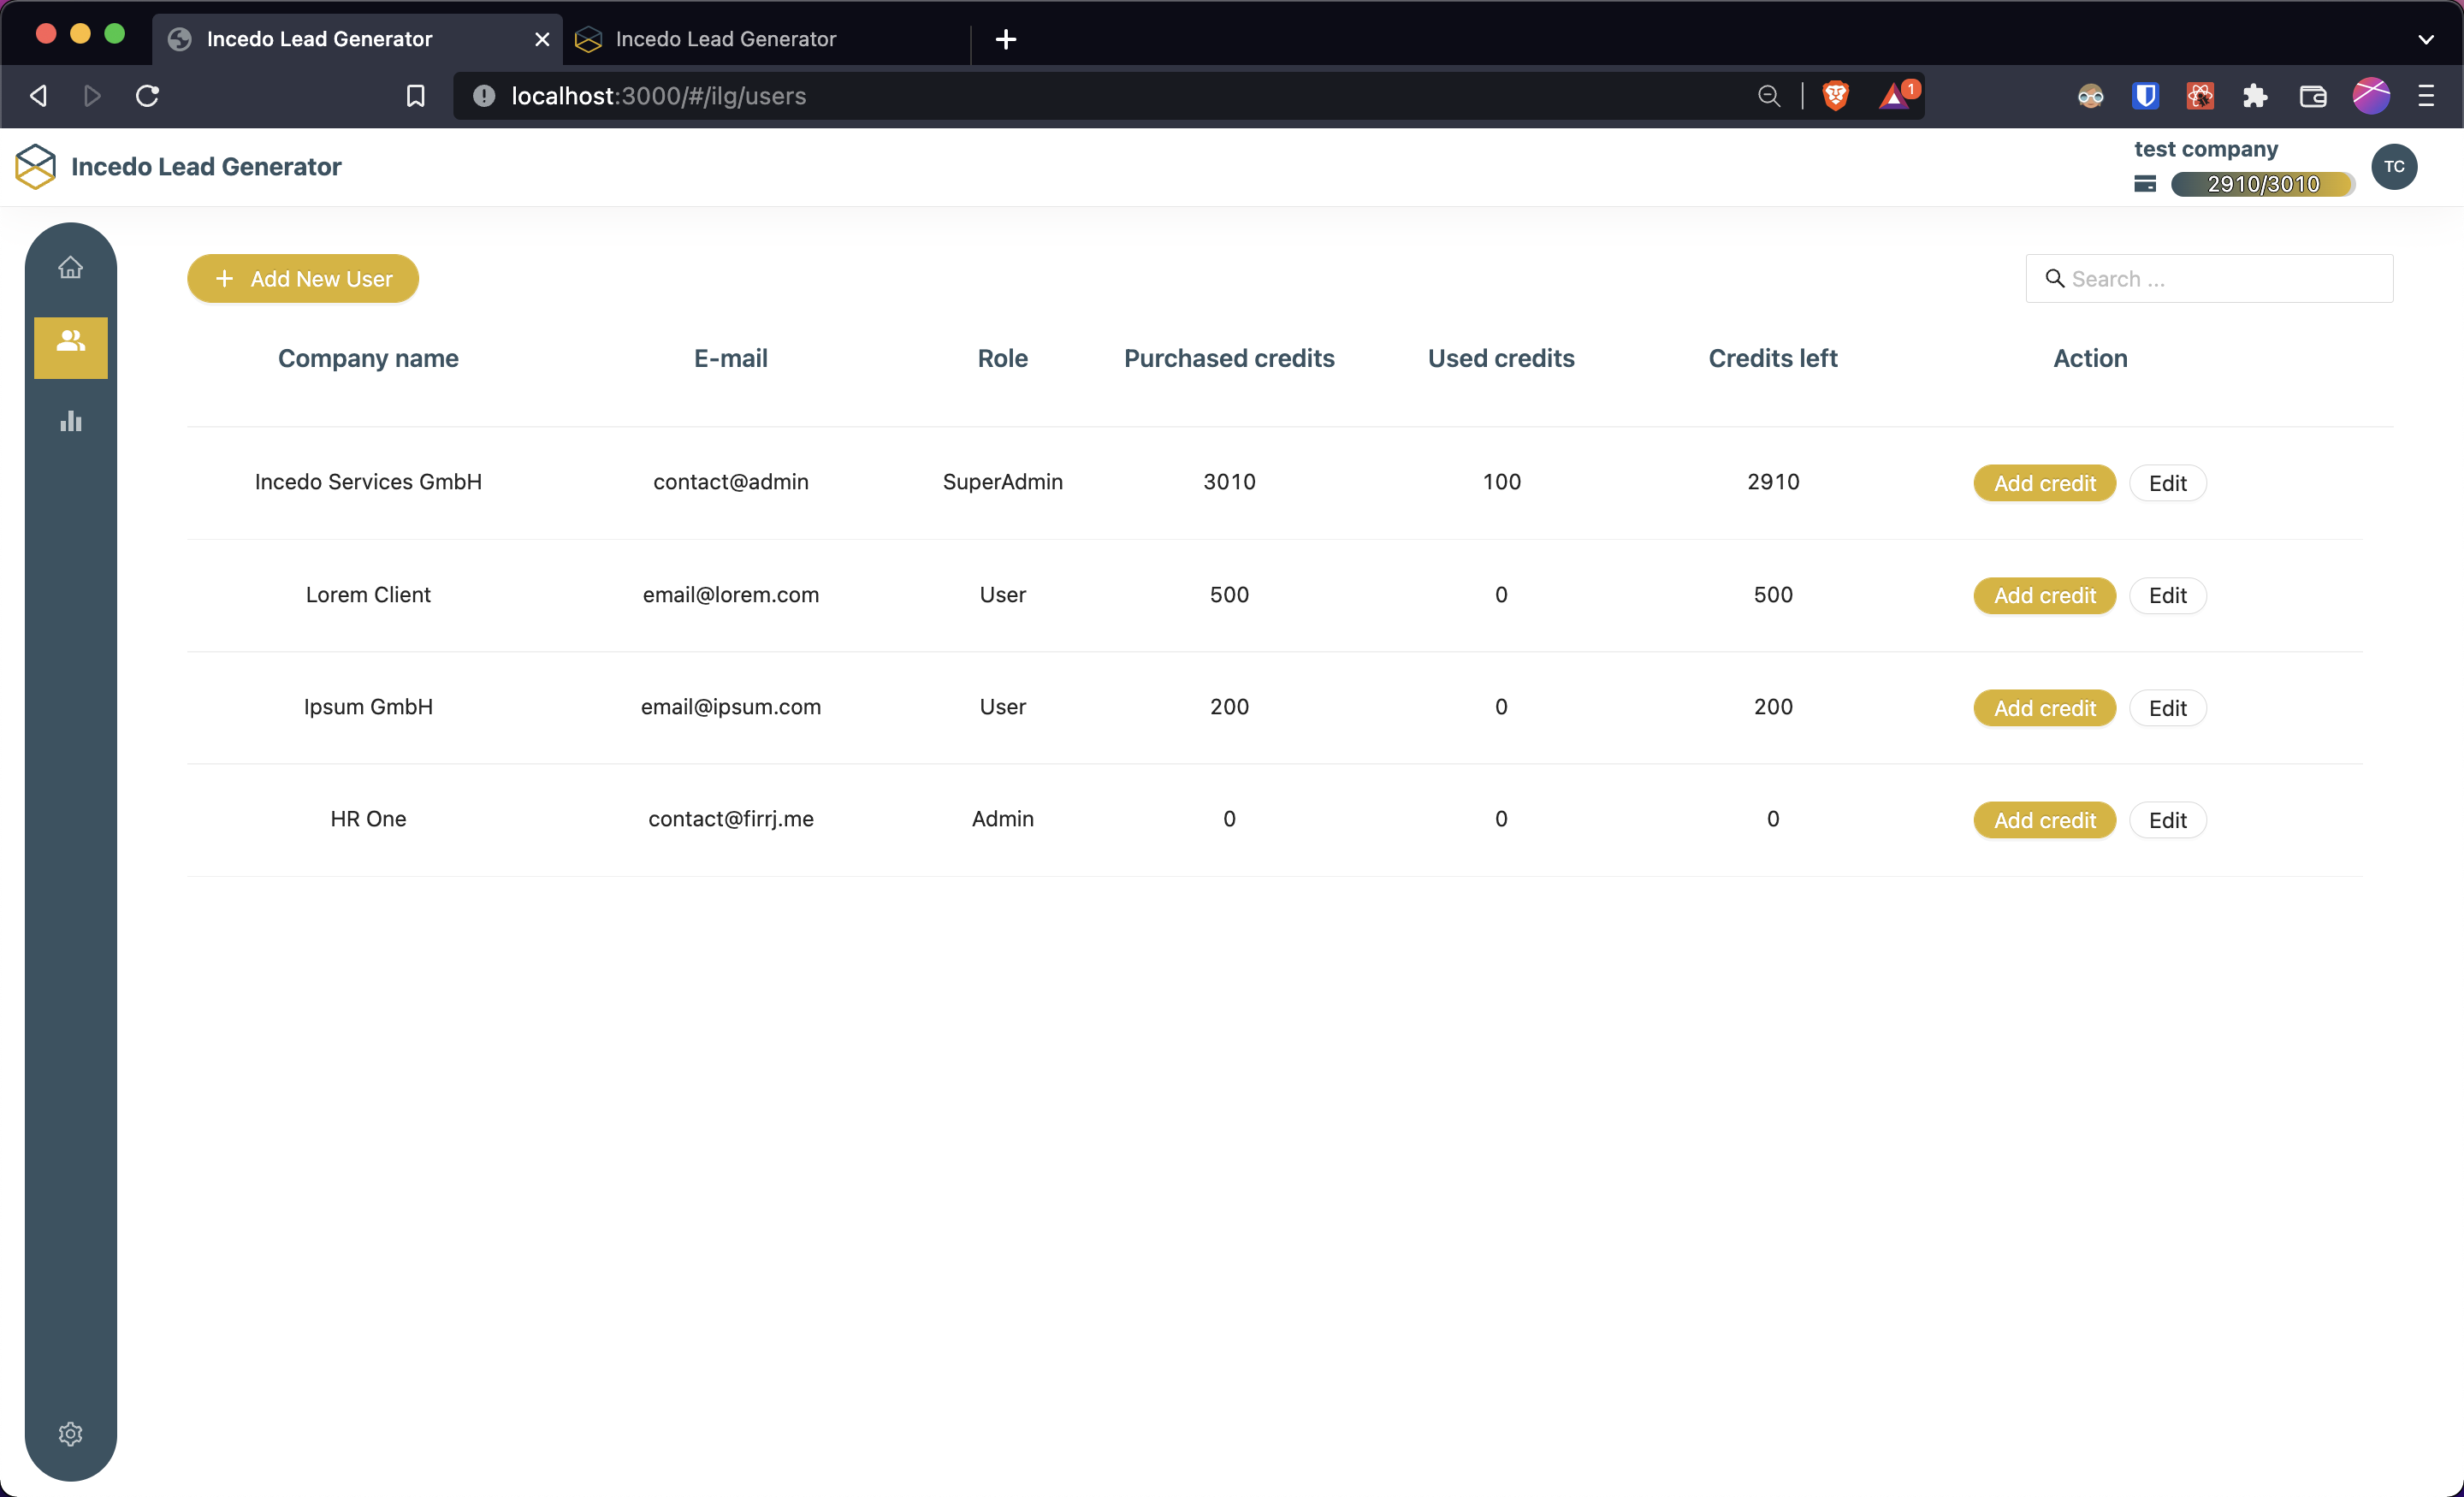
\includegraphics[width=\linewidth]{src/assets/app-screenshots/users.png}}
    \caption{View users page}
    \label{fig:users-view-page}
\end{figure}

In order to provide visibility to see whether leads are generated, we build on the legacy code by using a records system which is basically the increment of invites sent or leads generated each day.
\begin{figure}[H]
    \centering
    \makebox[\textwidth]{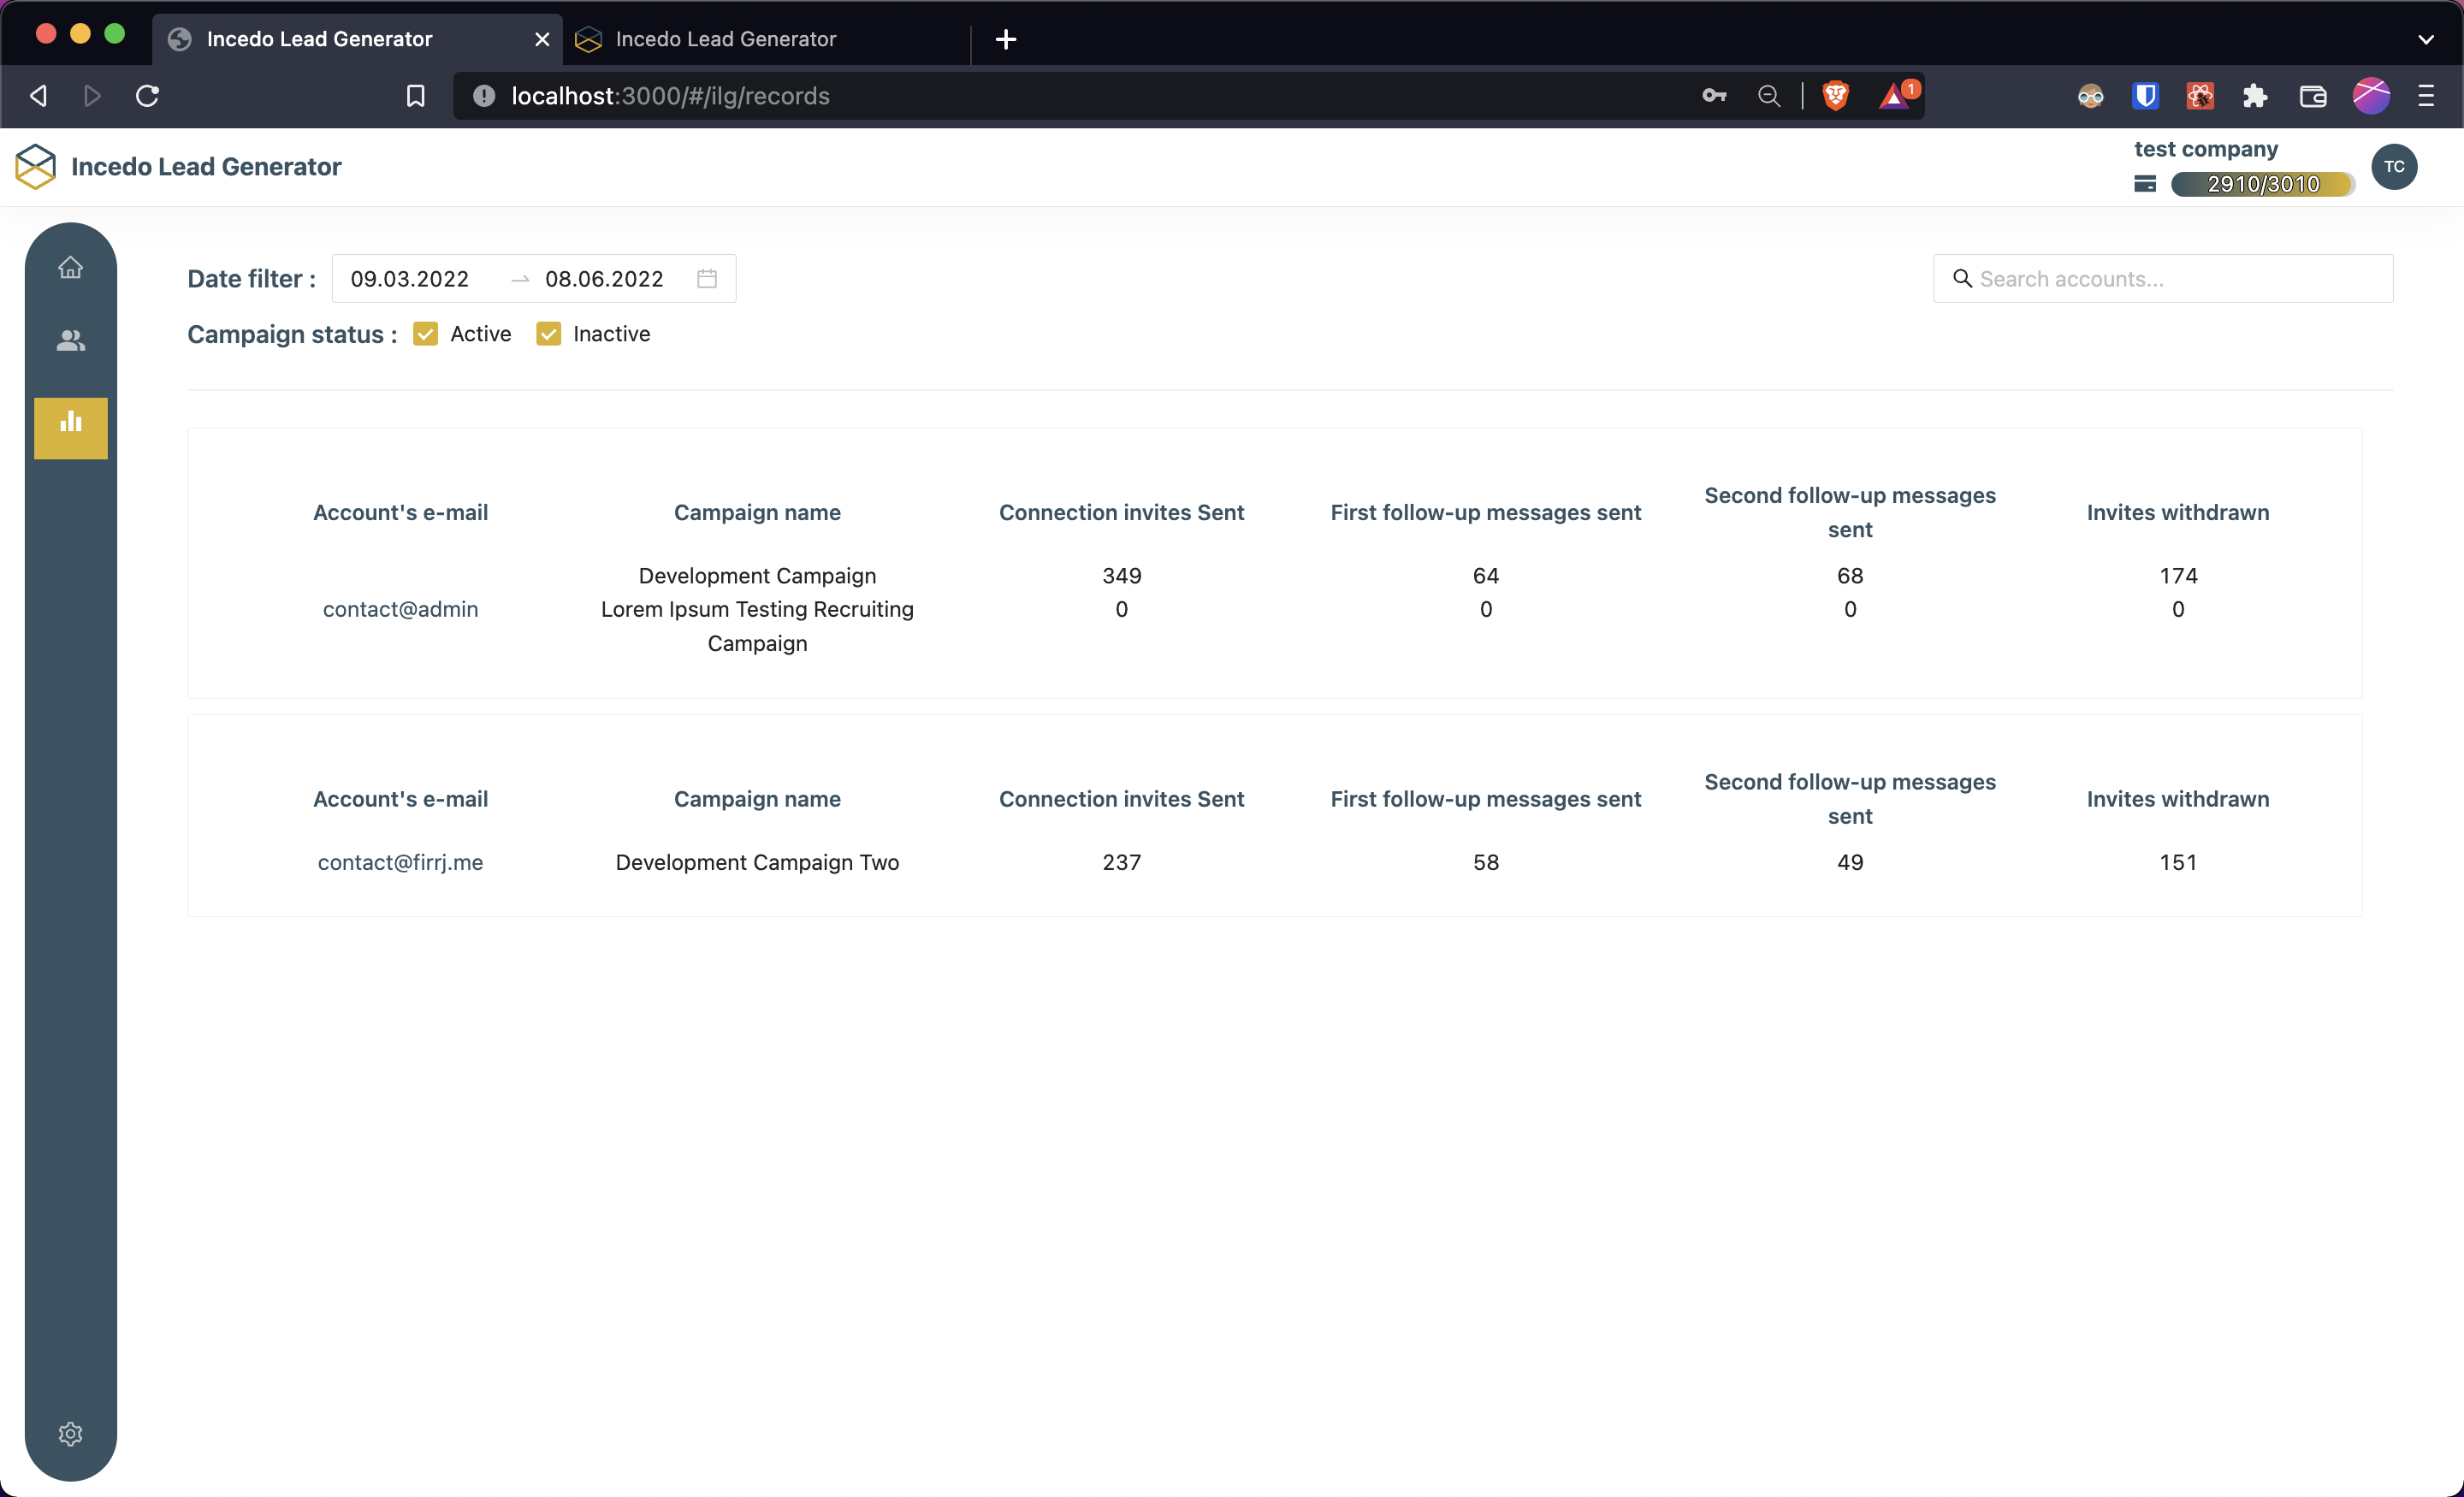
\includegraphics[width=\linewidth]{src/assets/app-screenshots/records.png}}
    \caption{Campaigns Records page}
    \label{fig:records-page}
\end{figure}

As seen from the screenshot, it is not easy on the eyes and the UI is very primitive.

We therefore implement an interactive good looking analytics dashboard with ChartJS in order to make it very easy for our client to keep an eye out on their campaigns and study their conversion rate to make changes if needed to number of invites and follow ups sent per day to improve the leads conversion.


\begin{figure}[H]
    \centering
    \makebox[\textwidth]{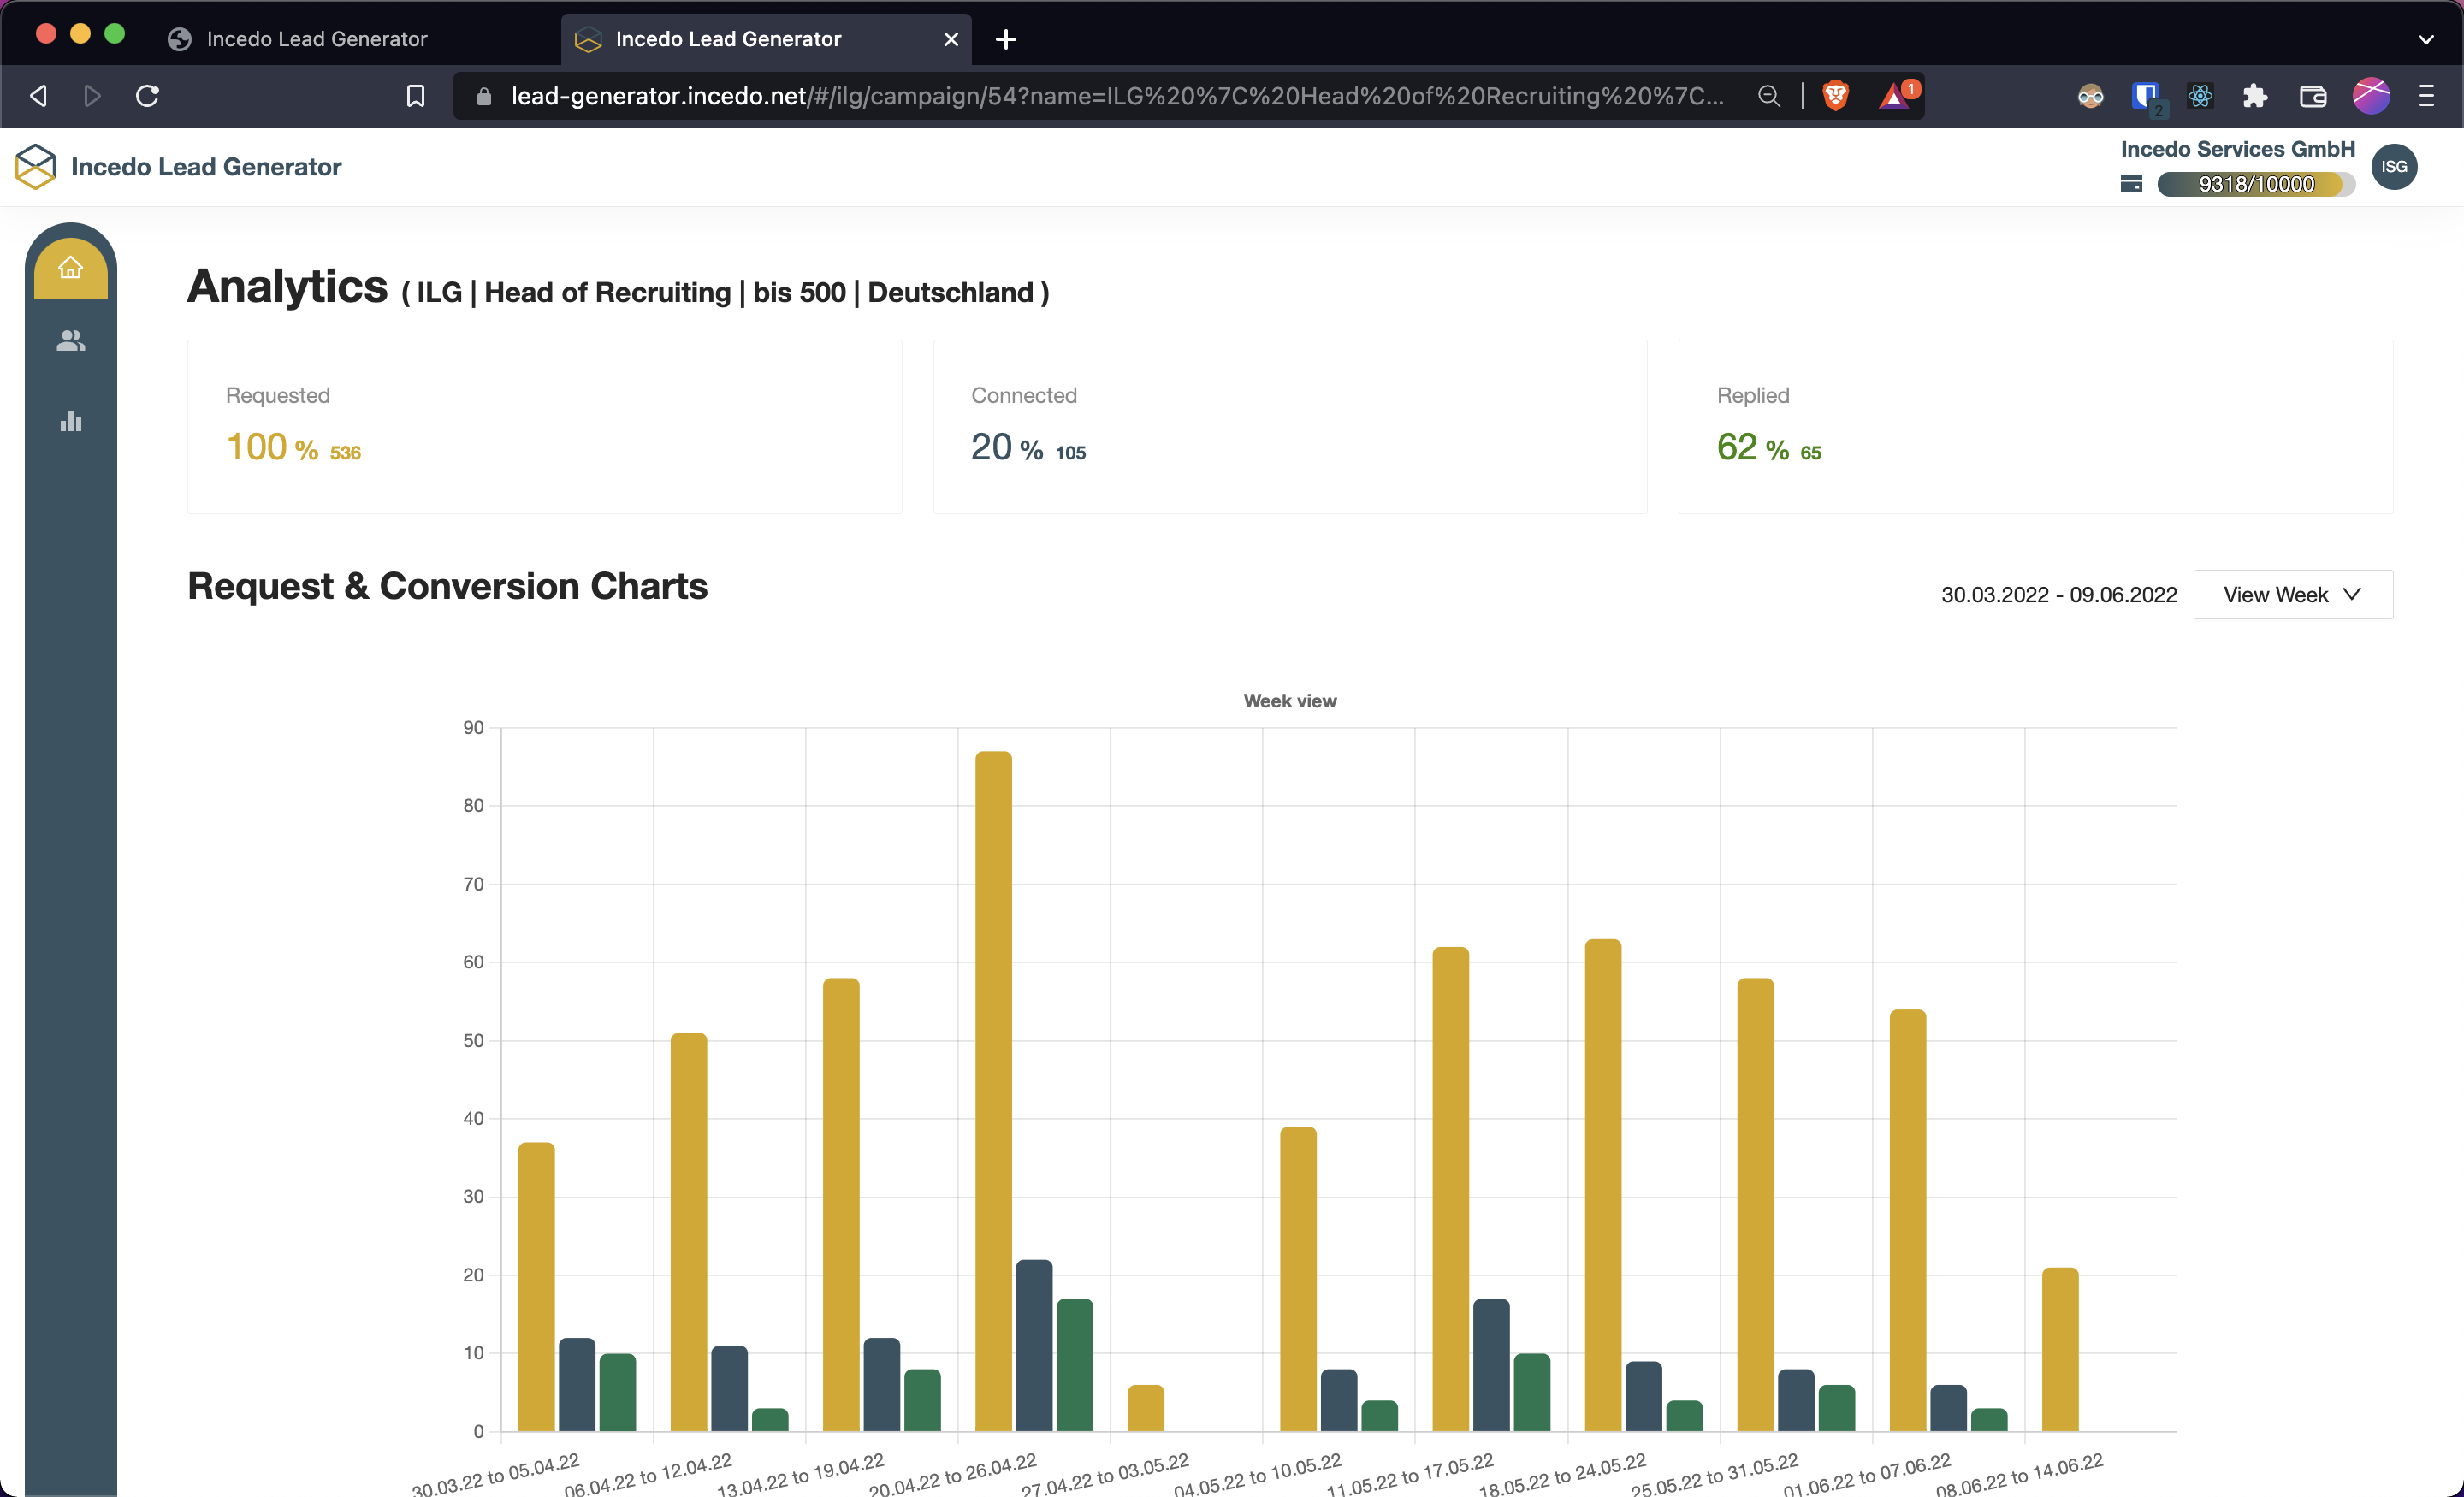
\includegraphics[width=\linewidth]{src/assets/app-screenshots/analytics-1.png}}
    \caption{Campaigns Analytics page}
    \label{fig:campaigns-analytics-page-1}
\end{figure}
\begin{figure}[H]
    \centering
    \makebox[\textwidth]{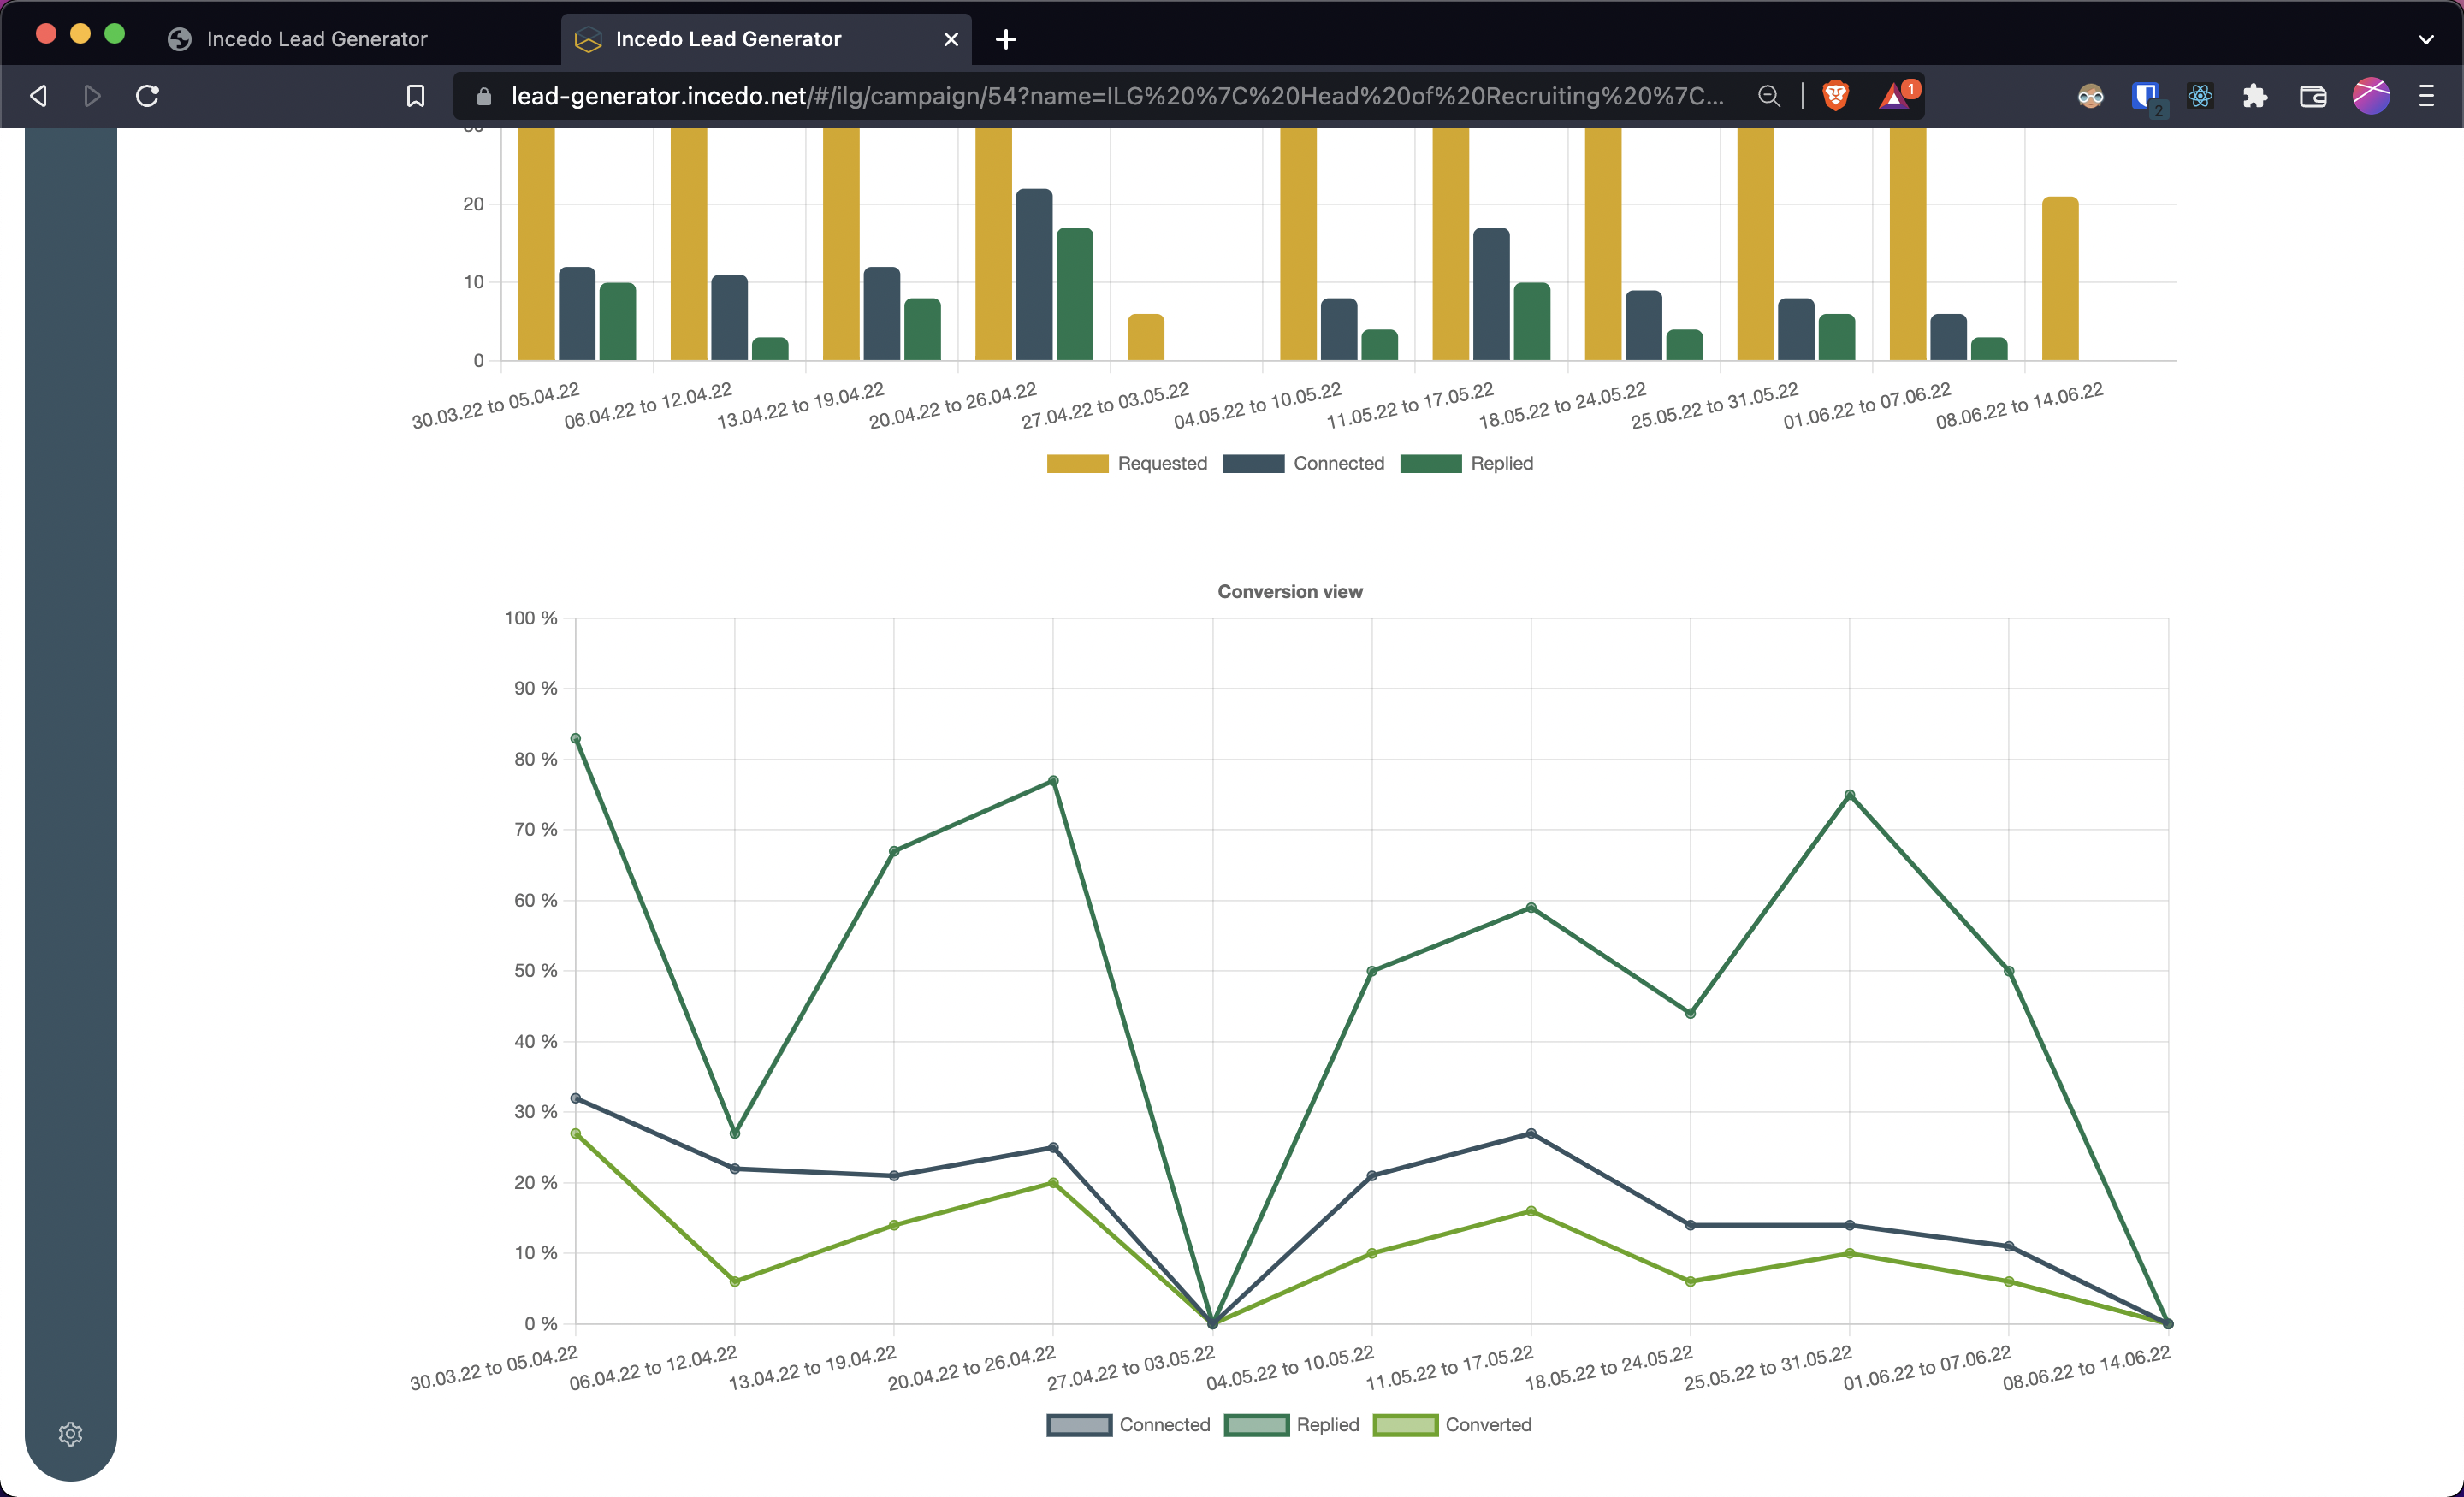
\includegraphics[width=\linewidth]{src/assets/app-screenshots/analytics-2.png}}
    \caption{Campaigns Analytics page}
    \label{fig:campaign-analytics-page-2}
\end{figure}
\newpage

% ----------------------- Monitoring ----------------------- %
\section{Monitoring}
The visibility definitely gets way better with dashboards.
Therefore, we also setup such monitoring solutions for our whole cluster.
The things we monitor vary from the cluster nodes' CPU and memory usage, to the logs of our microservices.

The first thing we do is exposing the dashboard provided by Kubernetes using manifest resources and kubectl.
Please see \textbf{Appendix d}.

\subsection{Monitoring the cluster nodes}
By using and configuring the Kubernetes community's Helm packages, we can very easily deploy what's called the \textbf{Kubernetes Prometheus Stack} which will give us access to the Grafana dashboard and to the Prometheus UI dashboard.

\subsubsection*{\underline{Prometheus}}
Prometheus is an open-source software used for event monitoring and alerting.
The way we do that is by collecting different kind of metrics and by configuring the automatic sending of alerts using rules in case of critical errors.
\begin{figure}[H]
    \centering
    \makebox[\textwidth]{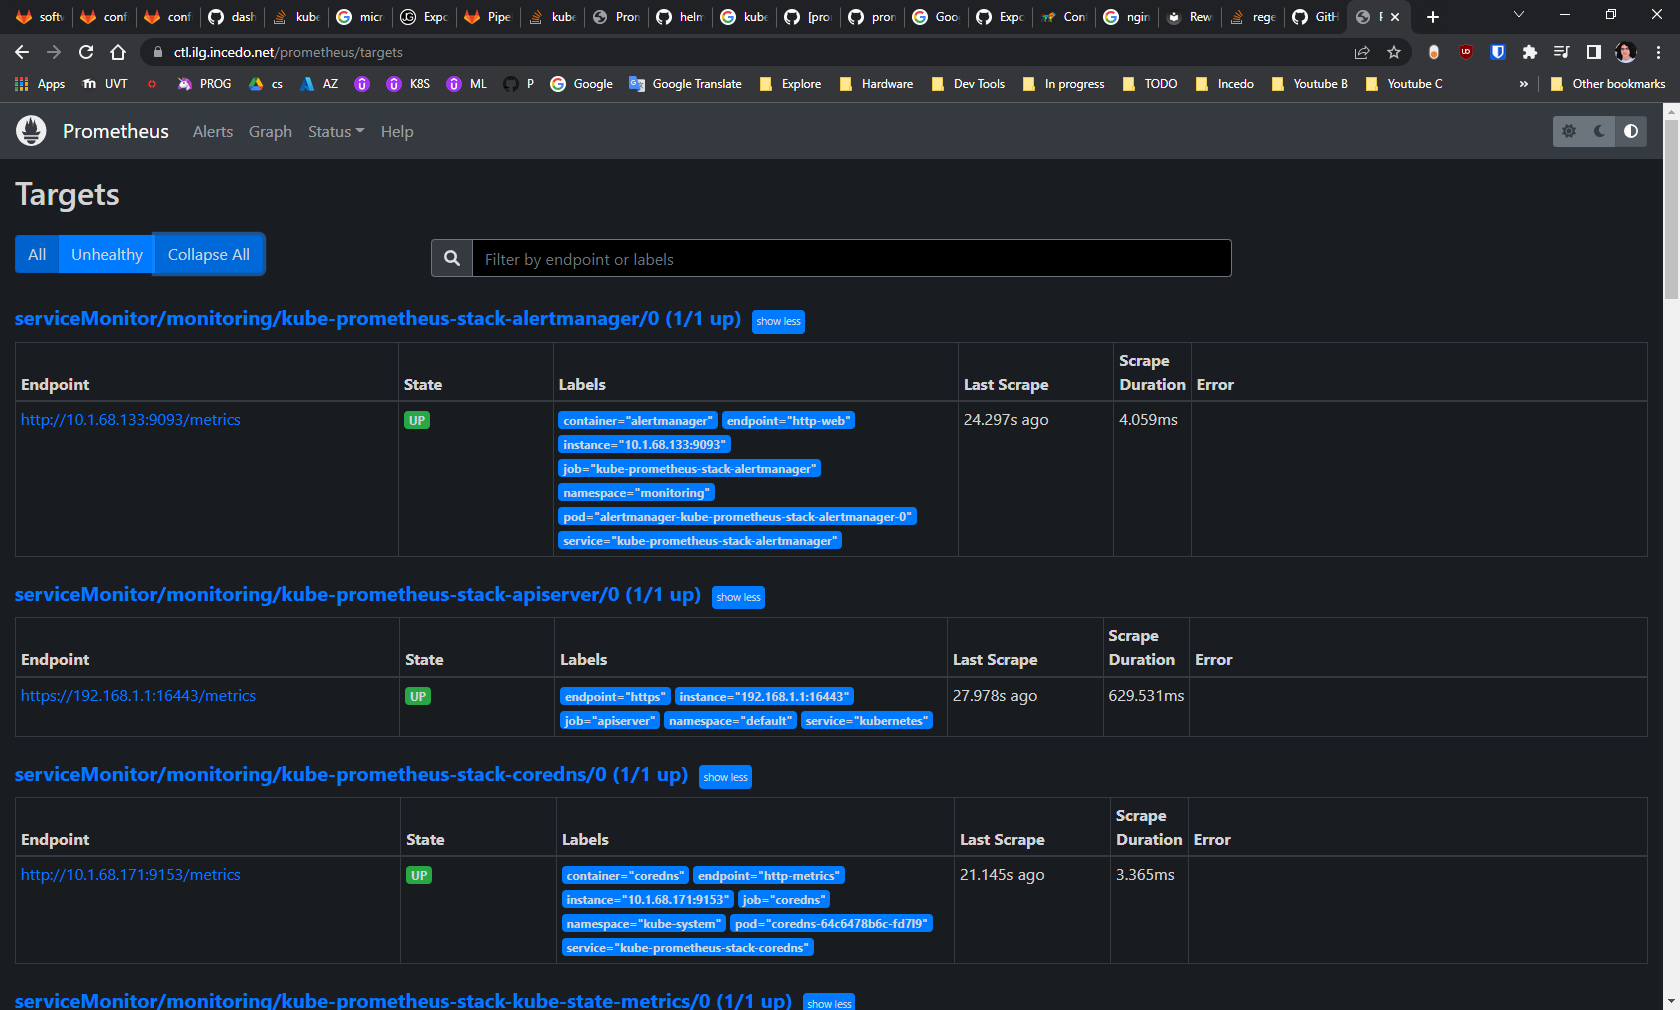
\includegraphics[width=\linewidth]{src/assets/images/prometheus-metrics.JPG}}
    \caption{Viewing the metrics endpoints with Prometheus UI}
    \label{fig:prometheus-ui-metrics-endpoint}
\end{figure}

\subsubsection*{\underline{Grafana}}
Grafana is an open-source interactive visualization web application.
We use it here to monitor our cluster nodes, and most importantly, the metrics of our application collected by Prometheus.
\begin{figure}[H]
    \centering
    \makebox[\textwidth]{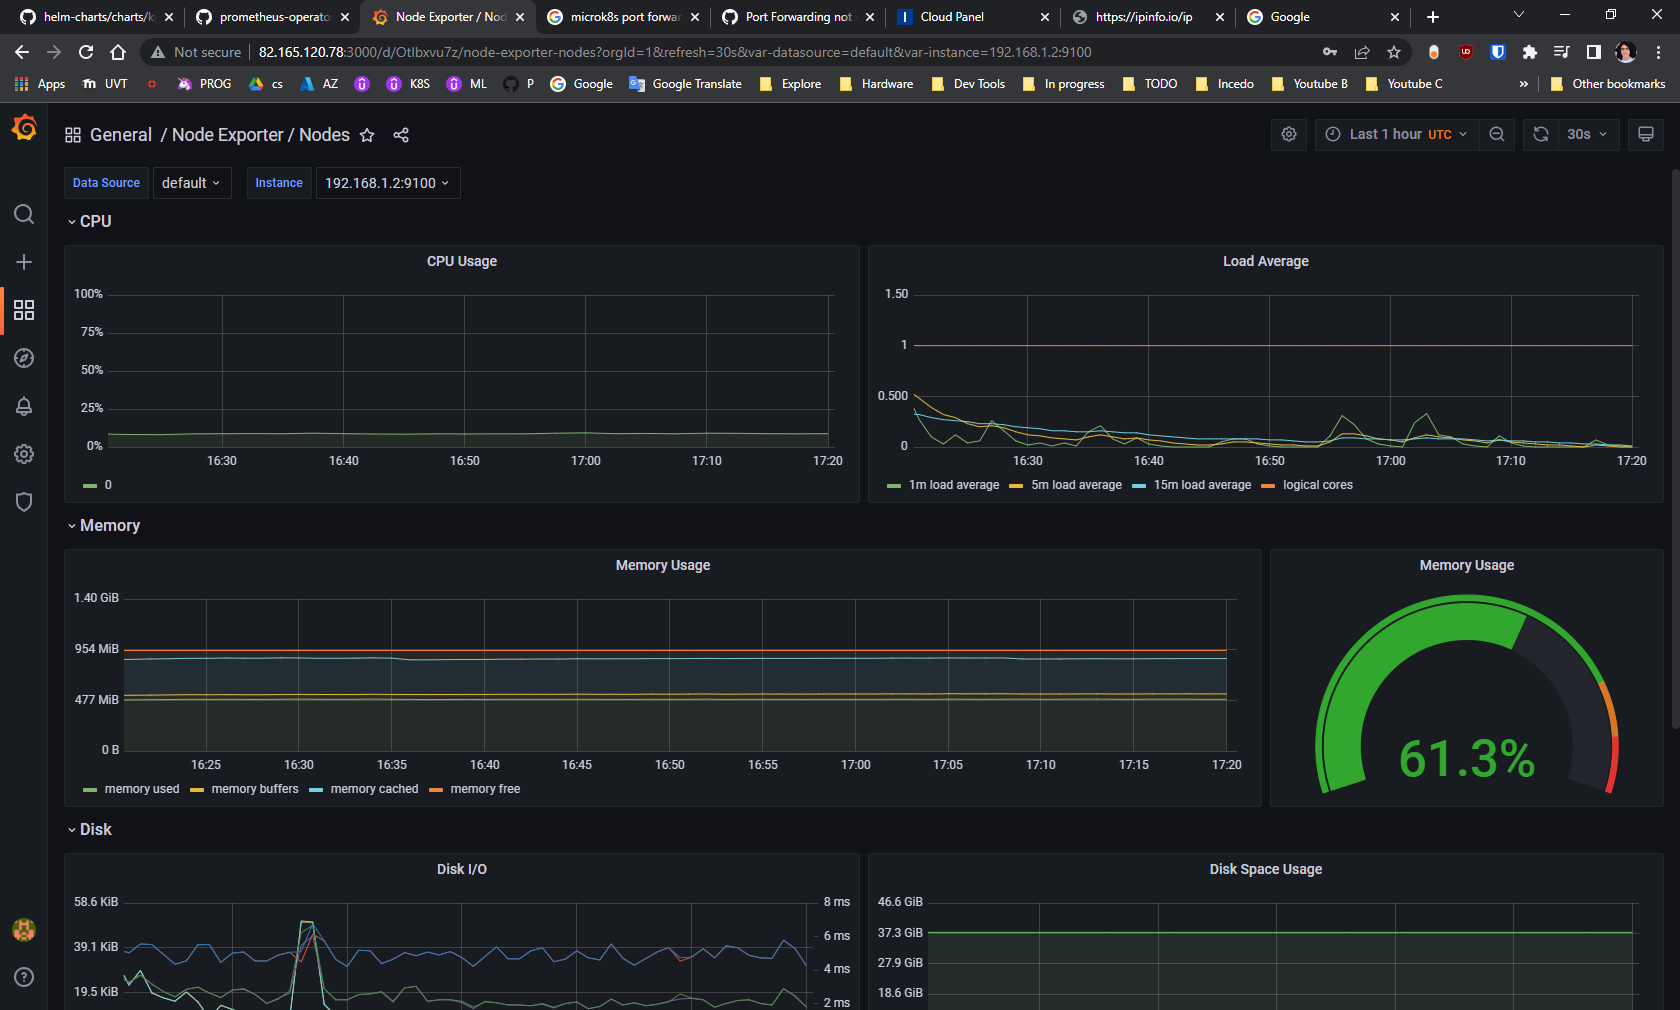
\includegraphics[width=\linewidth]{src/assets/images/grafana-nodes-monitoring.JPG}}
    \caption{Monitoring the cluster nodes with Grafana}
    \label{fig:grafana-node-monitoring}
\end{figure}

\subsection{Monitoring the logs}
In order to monitor the logs of our different microservices as well as any other applications running on the cluster efficiently, we need to

\begin{itemize}
    \item Collect the logs from the different Pods in the cluster
    \item Process and parse the logs to a uniform format, often json
    \item Send the logs to an indexing engine for easy querying
    \item We may also optionally create dashboards for our logs
\end{itemize}
The best way to go about doing this is by using the EFK Stack or more expressively the Elasticsearch, Fluentd and Kibana stack.

\subsubsection*{\underline{Elasticsearch \& Kibana}}
Elasticsearch is many things: it is often referred to as search engine, analytics engine or even a database and all of that is true.
It can process a huge amount of logs with relatively minimal resources and is therefore the optimal choice for our cluster.

Kibana is a data visualization dashboard exclusively used with Elasticsearch.
It is used almost always whenever there is an Elasticsearch instance involved.

By using the open-source \textbf{Elastic Stack Kubernetes Helm Charts}, we can create our Elasticsearch and Kibana setup in the cluster.
\begin{figure}[H]
    \centering
    \makebox[\textwidth]{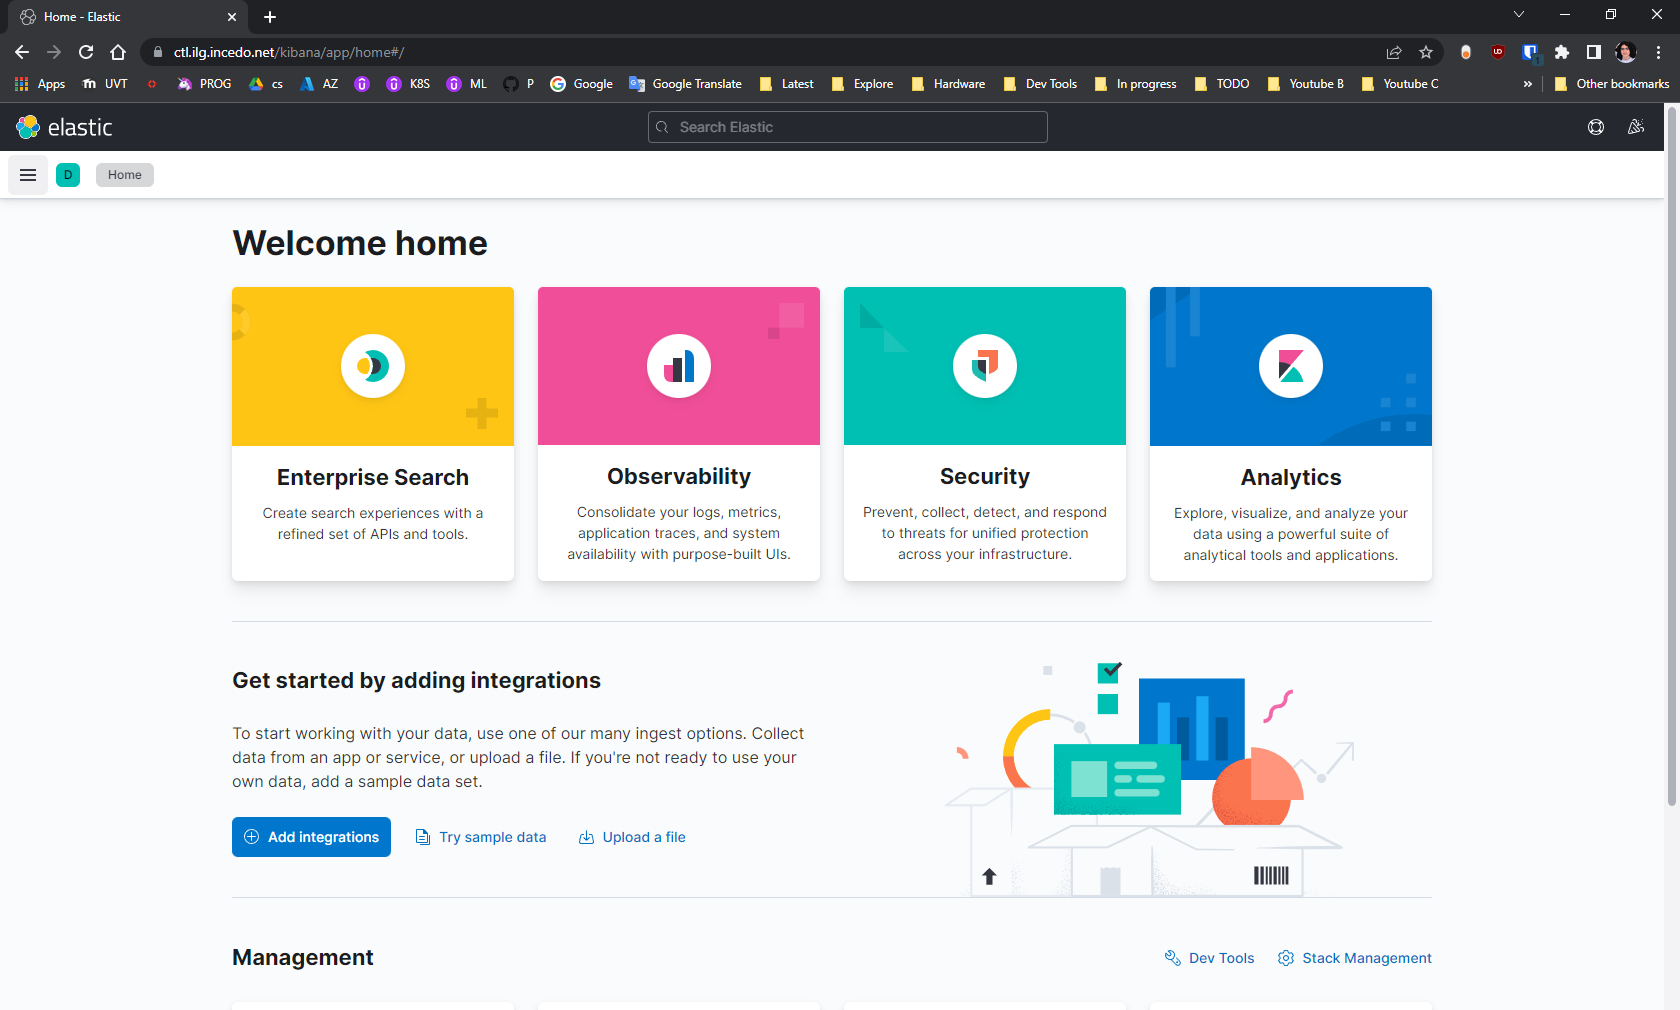
\includegraphics[width=\linewidth]{src/assets/images/kibana-home.JPG}}
    \caption{Kibana dashboard home screen}
    \label{fig:kibana-dashboard-home}
\end{figure}

\subsubsection*{\underline{Fluentd}}
Fluentd on the other hand is a data collector.
It runs in the background with the sole purpose of delivering the logs of all of our applications to any other service in a uniform way we specify.
We configure it to get the logs from the standard output of our Pods, parse them to json and send them to Elasticsearch.

We deploy Fluentd the manifest way, as opposed to using Helm Charts.
\begin{figure}[H]
    \centering
    \makebox[\textwidth]{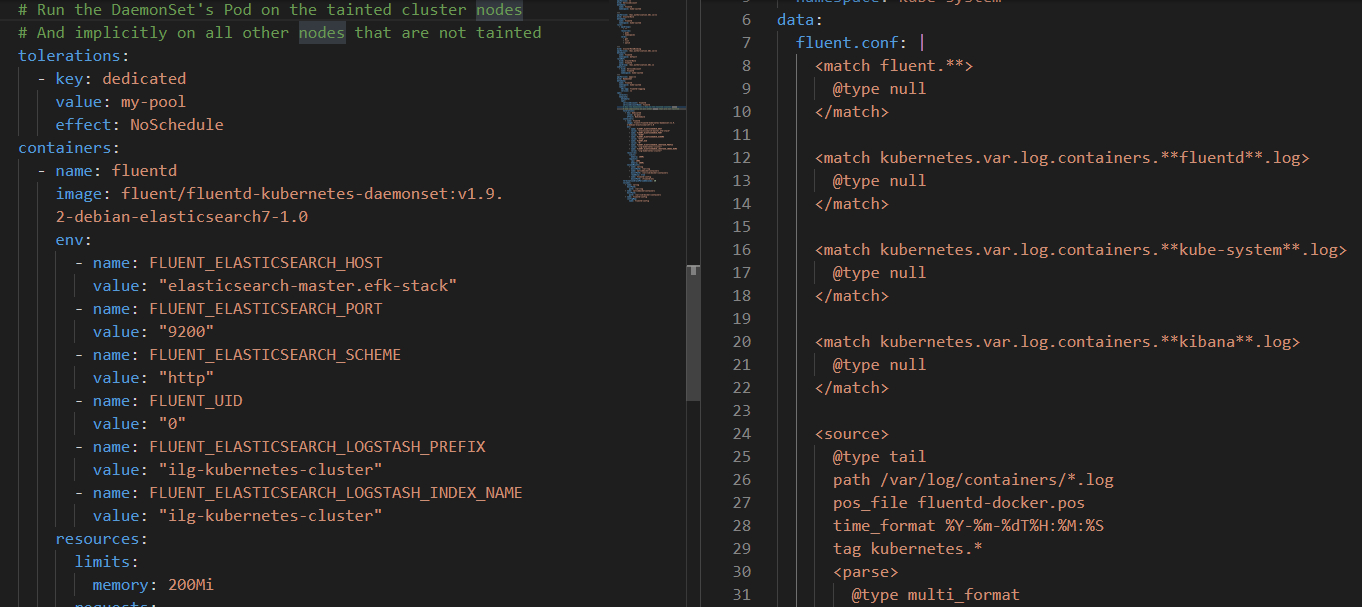
\includegraphics[width=\linewidth]{src/assets/images/fluentd-config-snippet.JPG}}
    \caption{Fluentd configuration extract}
    \label{fig:fluentd-config-snippet}
\end{figure}

And now we can finally use some of the advanced features of Elasticsearch such as the filtering and sorting of our logs from the Kibana dashboard.

\begin{figure}[H]
    \centering
    \makebox[\textwidth]{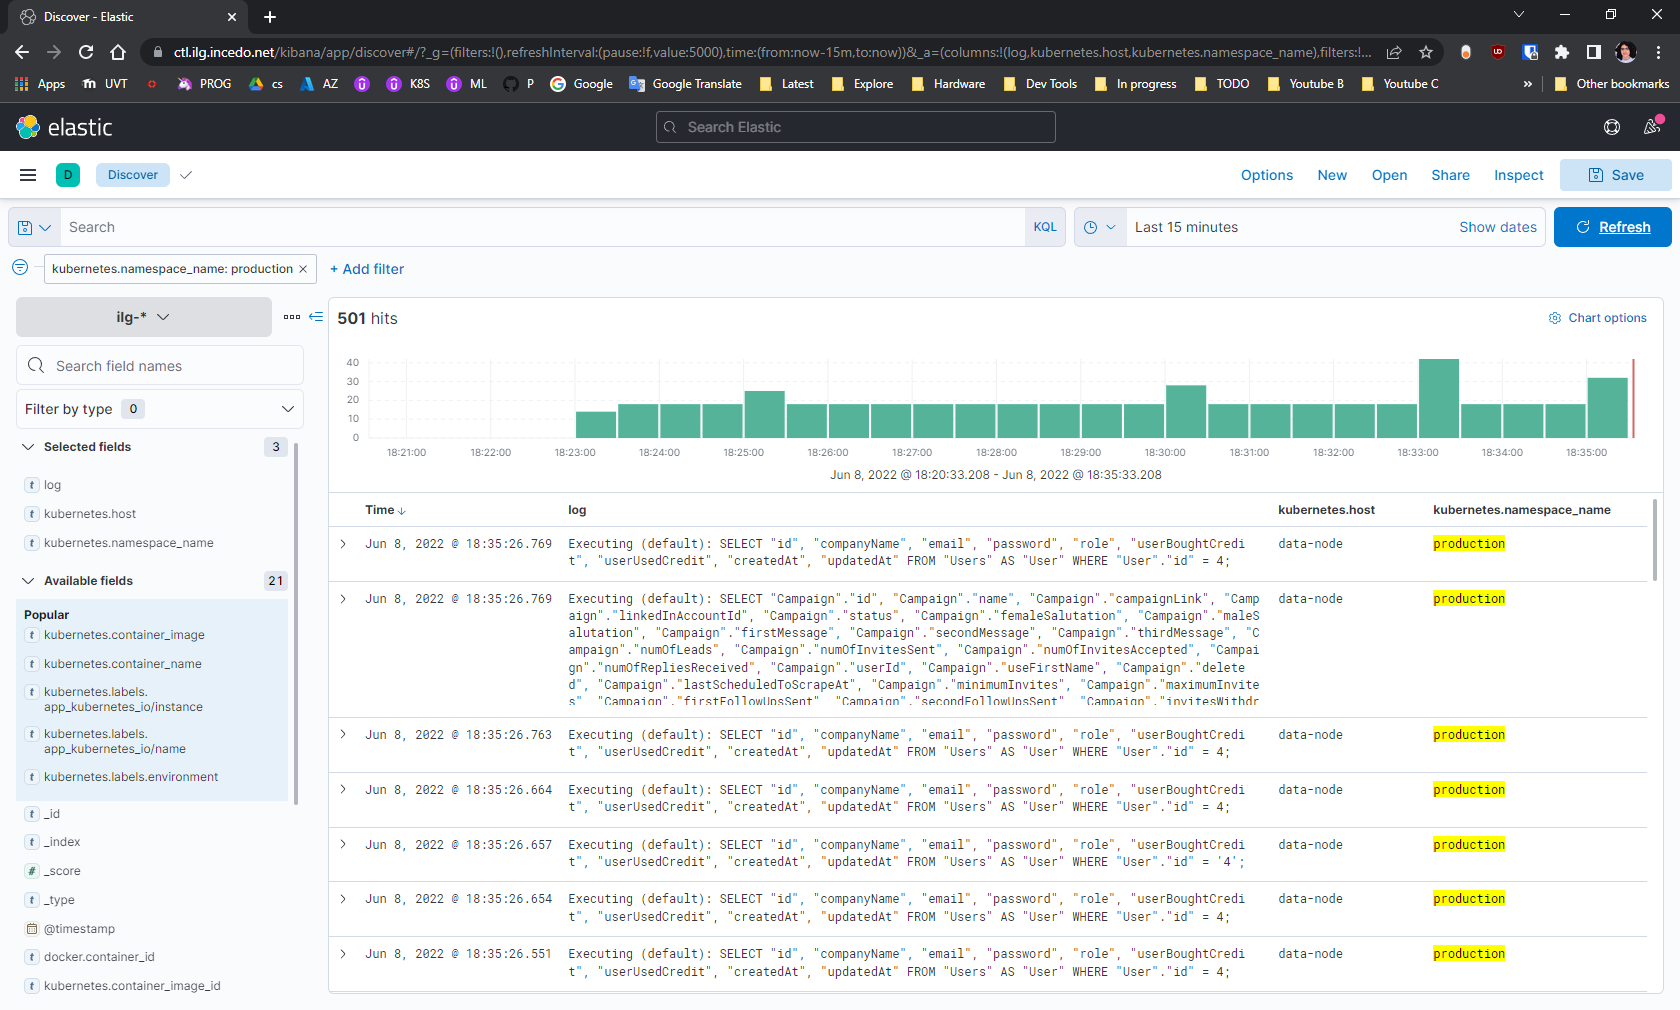
\includegraphics[width=\linewidth]{src/assets/images/efk-stack-logs.JPG}}
    \caption{Indexing the logs in Kibana}
    \label{fig:kibana-logs-indexing}
\end{figure}

\setcounter{secnumdepth}{0} % Set the section counter to 0 so next section is not counted in toc
% ----------------------- Conclusion ----------------------- %
\section{Conclusion}
A successful project comes from a successful development environment as well as a clean production environment with good and well thought of monitoring solutions.
For this reason, we spent quite a good amount of time setting up the infrastructure in a clean and scalable way using various tools and scripts which all conform to the modern ways of how DevOps should be done.
In the next chapter, we will list all of the technologies that we've used and also talk about the major difficulties that we've encountered in the whole making of the project.
